\documentclass[11pt,openany]{report}
\usepackage[margin=2.3cm]{geometry}
\usepackage{amsmath,amssymb,amsthm,mathtools}
\usepackage{graphicx,float,booktabs,array,enumitem,xcolor,caption,microtype}
\usepackage[most]{tcolorbox}
\usepackage[hidelinks]{hyperref}
\usepackage{lmodern}
\captionsetup{font=small,labelfont=bf}
\setlist{itemsep=2pt,topsep=4pt}
\graphicspath{{figs/}}
\setlength{\parskip}{0.35em}

\definecolor{keyc}{HTML}{EAF2FB}\definecolor{keyf}{HTML}{2A78D6}
\definecolor{recc}{HTML}{E8F7EF}\definecolor{recf}{HTML}{1BAF7A}
\definecolor{exc}{HTML}{FDF1EA}\definecolor{exf}{HTML}{EB6834}
\definecolor{warc}{HTML}{FBEAEA}\definecolor{warf}{HTML}{E34948}
\newtcolorbox{keyidea}[1][Key idea]{colback=keyc,colframe=keyf,boxrule=0.8pt,arc=3pt,fonttitle=\bfseries\small,title={#1},
  left=6pt,right=6pt,top=4pt,bottom=4pt}
\newtcolorbox{recipe}[1][Recipe]{colback=recc,colframe=recf,boxrule=0.8pt,arc=3pt,fonttitle=\bfseries\small,title={#1},
  left=6pt,right=6pt,top=4pt,bottom=4pt}
\newtcolorbox{worked}[1][Worked example]{colback=exc,colframe=exf,boxrule=0.8pt,arc=3pt,fonttitle=\bfseries\small,title={#1},
  left=6pt,right=6pt,top=4pt,bottom=4pt,breakable}
\newtcolorbox{pitfall}[1][Common pitfall]{colback=warc,colframe=warf,boxrule=0.8pt,arc=3pt,fonttitle=\bfseries\small,title={#1},
  left=6pt,right=6pt,top=4pt,bottom=4pt}
\newcommand{\R}{\mathbb{R}}
\newcommand{\tr}{\operatorname{tr}}
\newcommand{\eps}{\varepsilon}

\title{\textbf{Reading Dynamical Systems}\\[0.4em]
\large Fixed points, phase planes, bifurcations, hysteresis and slow--fast systems\\[0.2em]
\normalsize background material for the HSP--Epileptor work}
\author{}
\date{}

\begin{document}
\maketitle
\tableofcontents

%==========================================================================================
\chapter*{How to use this text}
\addcontentsline{toc}{chapter}{How to use this text}
%==========================================================================================
The goal is practical: to look at a set of equations, or at a phase portrait, and say what the system does and how
that behaviour can change. Three skills are built up in order.
\begin{enumerate}
\item \textbf{Reading a phase portrait} (Chapters 1--3): fixed points, their stability from the Jacobian, nullclines,
limit cycles.
\item \textbf{Recognising bifurcations} (Chapters 4--7): how a fixed point or a cycle appears, disappears or changes
stability when a parameter moves, with the fingerprints that identify each one (how amplitude and frequency scale near
it), and the hysteresis they can create.
\item \textbf{Slow--fast systems} (Chapters 8--9): systems where one variable is much slower than the others, which is
the structure of bursting neurons and of the Epileptor.
\end{enumerate}
Chapter 10 collects the procedures into one checklist, Chapter 11 applies everything to the Epileptor, and the
appendix has exercises with solutions. Every figure is computed from the equation printed next to it
(\texttt{figures.py}). The standard references, for more depth, are Strogatz \cite{strogatz} (the most readable),
Izhikevich \cite{izhikevich} (neuron-oriented, with the onset/offset classification used here), Kuznetsov \cite{kuznetsov}
(rigorous) and Kuehn \cite{kuehn} (slow--fast systems).

\textbf{Notation and drawing conventions.} $\dot x = dx/dt$. A \emph{parameter} ($\mu$, $a$, $I$, $x_0$) is held constant
while we study the dynamics and is varied only to see how the dynamics change. In every figure:
\begin{center}\small
\begin{tabular}{ll}
\toprule
filled circle & stable fixed point (attracts nearby states) \\
open circle & unstable fixed point (repels in at least one direction) \\
grey circle & the degenerate point at a bifurcation \\
solid curve in a bifurcation diagram & stable branch \\
dashed curve & unstable branch \\
grey stream lines & direction of the flow \\
\bottomrule
\end{tabular}
\end{center}

%==========================================================================================
\chapter{One-dimensional flows: reading the phase line}
%==========================================================================================
\section{The phase line}
A one-dimensional system $\dot x = f(x)$ assigns a velocity to every point of the line. Its whole behaviour can be read
from the graph of $f$ (Fig.~\ref{fig:phaseline}a):
\begin{itemize}
\item where $f(x) > 0$, $x$ increases: the flow points right;
\item where $f(x) < 0$, $x$ decreases: the flow points left;
\item where $f(x^*) = 0$, $x$ does not move: $x^*$ is a \textbf{fixed point} (equilibrium, steady state).
\end{itemize}
A fixed point is \textbf{stable} if the arrows on both sides point towards it, and \textbf{unstable} if at least one
side points away. Nothing else can happen in one dimension: a trajectory moves monotonically towards a fixed point or
towards infinity. It can never turn around, because to turn around it would have to pass through $f = 0$, which is a
fixed point where it would stop. \emph{One-dimensional systems cannot oscillate.}

\begin{figure}[H]\centering
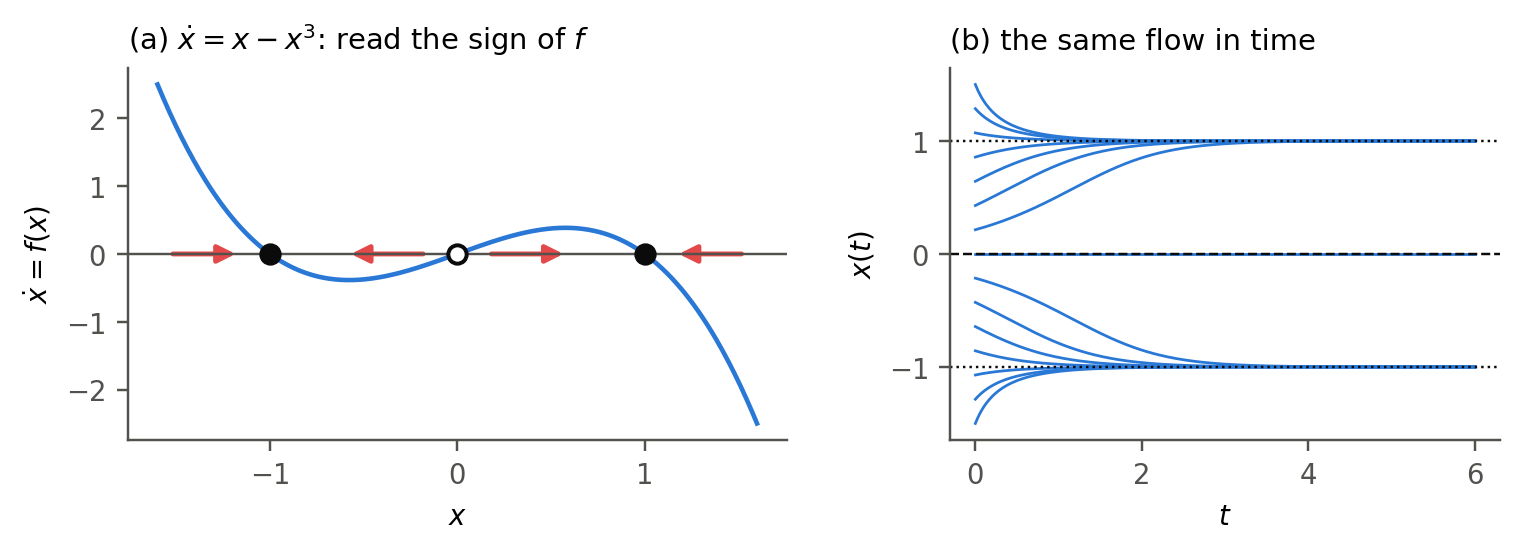
\includegraphics[width=0.95\linewidth]{f01_phaseline.png}
\caption{(a) $\dot x = x - x^3$: three fixed points, $x^*=-1$ and $1$ stable, $0$ unstable. The red arrows give the
direction of motion read from the sign of $f$. (b) Trajectories from 15 initial conditions: each settles on the
nearest stable fixed point; the unstable one at 0 separates the two \emph{basins of attraction}.}\label{fig:phaseline}
\end{figure}

\section{Linear stability}
Near a fixed point, write $x = x^* + u$ with $u$ small and expand $f$:
\[
\dot u = f(x^* + u) = \underbrace{f(x^*)}_{=0} + f'(x^*)\,u + O(u^2) \quad\Rightarrow\quad u(t) \approx u(0)\,e^{f'(x^*)\,t}.
\]
\begin{keyidea}
The slope $\lambda = f'(x^*)$ is the \textbf{eigenvalue} of the fixed point. $\lambda<0$: perturbations decay at rate
$|\lambda|$, so the fixed point is stable and $1/|\lambda|$ is its relaxation time. $\lambda>0$: perturbations grow, so it
is unstable. $\lambda = 0$: linearisation says nothing, and this is exactly where bifurcations happen.
\end{keyidea}
For $f = x - x^3$: $f'(x) = 1 - 3x^2$, so $f'(0) = 1$ (unstable) and $f'(\pm1) = -2$ (stable), as in the figure. A
graphical rule that is worth memorising: \emph{a fixed point where $f$ crosses zero going down is stable; going up,
unstable.}

\section{Potentials}
Any one-dimensional flow can be written as $\dot x = -dV/dx$ with $V(x) = -\int f\,dx$. The state rolls downhill on $V$:
minima of $V$ are stable fixed points and maxima are unstable ones. For $f = x - x^3$, $V = -x^2/2 + x^4/4$, a double
well. Thinking of the potential helps intuition for bistability (two wells) and for bifurcations (a well flattens and
disappears), but it does not exist in general for two or more variables, so the rest of the text uses the flow directly.

%==========================================================================================
\chapter{Two-dimensional linear systems and the Jacobian}
%==========================================================================================
\section{Linearisation in two dimensions}
For $\dot x = f(x,y)$, $\dot y = g(x,y)$, a fixed point $(x^*,y^*)$ solves $f = g = 0$. Writing small deviations
$\mathbf u = (x - x^*, y - y^*)$ and expanding to first order gives $\dot{\mathbf u} = J\,\mathbf u$ with the
\textbf{Jacobian}
\[
J = \begin{pmatrix} \partial_x f & \partial_y f\\ \partial_x g & \partial_y g\end{pmatrix}_{(x^*,y^*)} .
\]
The solutions of the linear system are combinations of $e^{\lambda t}\mathbf v$, where $\lambda$ are the eigenvalues
of $J$ and $\mathbf v$ its eigenvectors. With the trace $\tau = \tr J$ and the determinant $\Delta = \det J$,
\[
\lambda_{1,2} = \frac{\tau}{2} \pm \sqrt{\frac{\tau^2}{4} - \Delta},\qquad \lambda_1 + \lambda_2 = \tau,\qquad \lambda_1\lambda_2 = \Delta .
\]
So two numbers, $\tau$ and $\Delta$, decide everything (Fig.~\ref{fig:td}).

\begin{figure}[H]\centering
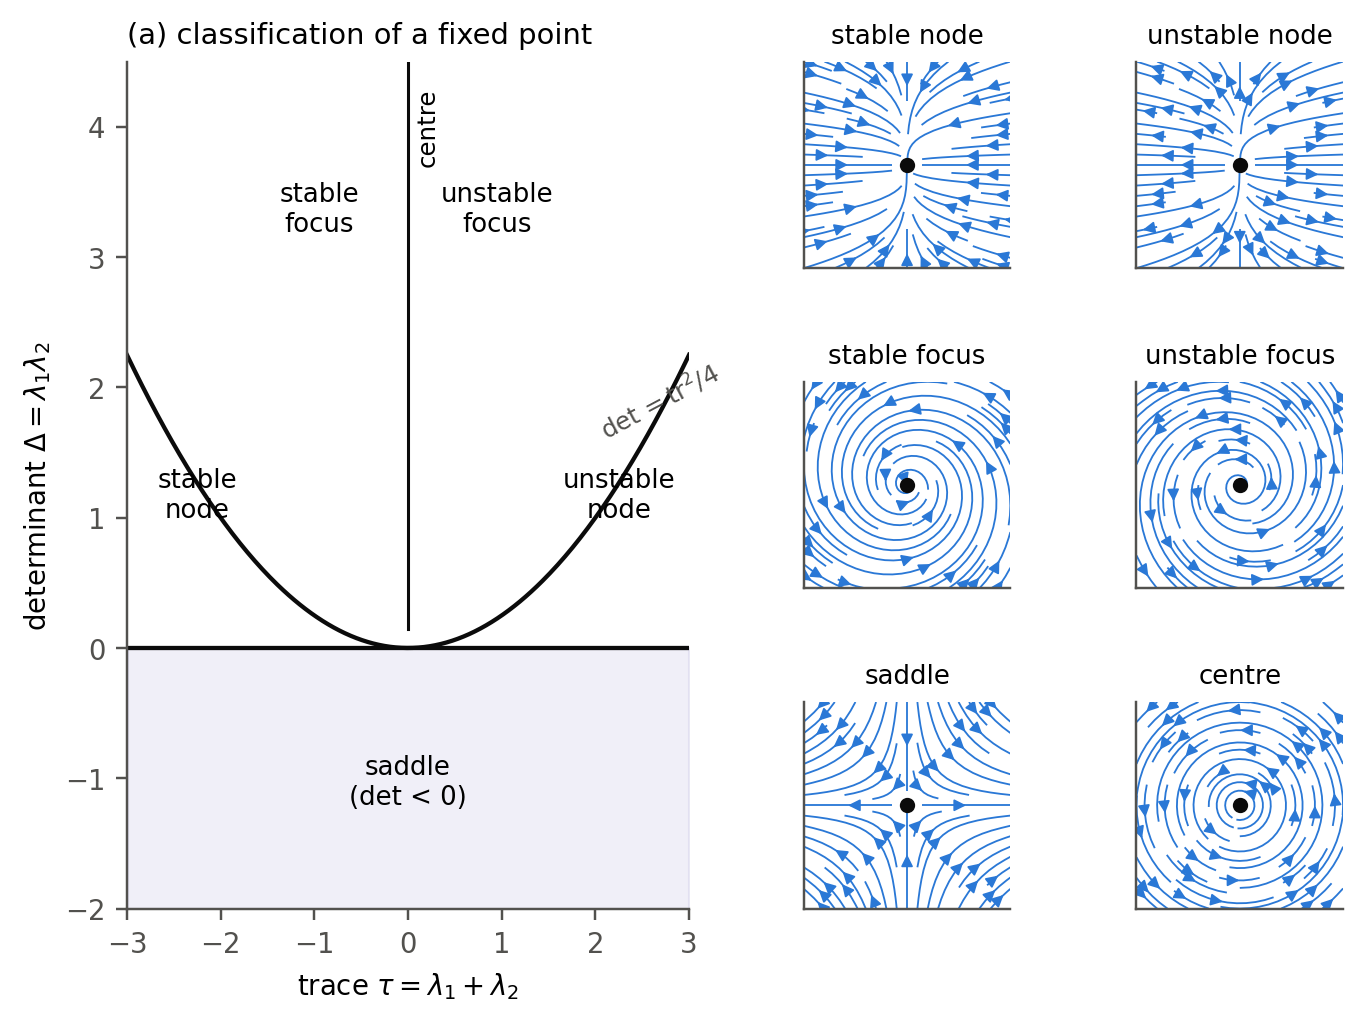
\includegraphics[width=0.95\linewidth]{f02_tracedet.png}
\caption{(a) The trace--determinant plane. (b) The flow near each kind of fixed point.}\label{fig:td}
\end{figure}

\begin{center}\small
\begin{tabular}{>{\raggedright}p{3.1cm}>{\raggedright}p{3.6cm}p{7.2cm}}
\toprule
condition & eigenvalues & name and behaviour \\
\midrule
$\Delta < 0$ & real, opposite signs & \textbf{saddle}: attracts along one direction, repels along the other. Always unstable.\\
$\Delta>0$, $\tau<0$, $\tau^2>4\Delta$ & real, both negative & \textbf{stable node}: approached without turning. \\
$\Delta>0$, $\tau<0$, $\tau^2<4\Delta$ & complex, $\mathrm{Re}<0$ & \textbf{stable focus} (spiral): damped oscillation around it, frequency $\sqrt{\Delta - \tau^2/4}$. \\
$\Delta>0$, $\tau>0$ & $\mathrm{Re}>0$ & \textbf{unstable node} or \textbf{unstable focus}. \\
$\Delta>0$, $\tau=0$ & purely imaginary & \textbf{centre} for the linear system; for the nonlinear one, undecided (this is the Hopf condition). \\
$\Delta = 0$ & one zero eigenvalue & degenerate; this is the saddle-node condition. \\
\bottomrule
\end{tabular}
\end{center}

\begin{keyidea}[Two lines in the trace--determinant plane are bifurcations]
As a parameter changes, the fixed point moves in the $(\tau,\Delta)$ plane. It can lose stability in only two ways:
\begin{itemize}
\item by crossing $\Delta = 0$: a real eigenvalue passes through zero (\textbf{saddle-node} family, Chapter 4);
\item by crossing $\tau = 0$ with $\Delta>0$: a complex pair crosses the imaginary axis (\textbf{Hopf}, Chapter 5).
\end{itemize}
Everything about local bifurcations of fixed points in two dimensions follows from this.
\end{keyidea}

\section{Saddles and their manifolds}
A saddle has two special trajectories through it: the \textbf{stable manifold} $W^s$ (the curve along which states
approach the saddle, tangent to the eigenvector with $\lambda<0$) and the \textbf{unstable manifold} $W^u$ (along which
they leave, tangent to the eigenvector with $\lambda>0$). The stable manifold of a saddle is a \textbf{separatrix}:
states on its two sides go to different places. In excitable neurons the stable manifold of a saddle is the
\emph{threshold}. These manifolds also drive the global bifurcations of Chapter 6: when $W^u$ of a saddle comes back to
the saddle along $W^s$, a homoclinic loop forms.

\begin{pitfall}
A saddle looks unimportant because nothing ever sits on it. It is the opposite: saddles organise phase space. Their
stable manifolds are thresholds and basin boundaries; their collisions with nodes (saddle-node) and with cycles
(homoclinic) are how rest states and oscillations are destroyed.
\end{pitfall}

%==========================================================================================
\chapter{Reading a phase plane}
%==========================================================================================
\section{Nullclines}
The \textbf{$x$-nullcline} is the curve where $\dot x = f(x,y) = 0$: there the flow is purely vertical. The
\textbf{$y$-nullcline} is where $\dot y = 0$: there the flow is purely horizontal. Fixed points are the intersections of
the two nullclines. Drawing them is the single most useful step in reading a two-dimensional system, because they cut
the plane into regions in which the signs of $\dot x$ and $\dot y$ are constant.

\begin{recipe}[Reading a phase plane]
\begin{enumerate}
\item Draw the $x$-nullcline ($f=0$) and the $y$-nullcline ($g=0$).
\item In each region between them, find the signs of $\dot x$ and $\dot y$ (test one point). The flow points
NE, NW, SE or SW accordingly; on an $x$-nullcline it points straight up or down, on a $y$-nullcline straight left or
right.
\item Mark the intersections (fixed points). Classify each with $\tau$ and $\Delta$ of the Jacobian.
\item Look for closed regions the flow cannot leave. If such a region contains no stable fixed point, it contains a
limit cycle (Poincaré--Bendixson theorem, \S\ref{sec:pb}).
\item Find the saddles and sketch their stable manifolds: these are the thresholds.
\end{enumerate}
\end{recipe}

\section{Stability from the geometry of the nullclines}
At a fixed point, the slopes of the two nullclines already contain the determinant. Along the $x$-nullcline,
$f_x\,dx + f_y\,dy = 0$, so its slope is $m_f = -f_x/f_y$; likewise $m_g = -g_x/g_y$. Then
\[
\Delta = f_x g_y - f_y g_x = f_y\,g_y\,(m_g - m_f).
\]
So the sign of $\Delta$ is decided by which nullcline is steeper at the crossing (and by the signs of $f_y$, $g_y$). In
particular, \textbf{when two nullclines touch tangentially, $m_f = m_g$ and $\Delta = 0$}: this is a saddle-node. When
a parameter makes the nullclines pull apart after touching, two fixed points have merged and disappeared. For the
FitzHugh--Nagumo model below, $f_y = -1$ and $g_y = -\eps b<0$, so $\Delta>0$ whenever the $y$-nullcline is steeper
than the $x$-nullcline at the crossing.

\section{An example to practise on: FitzHugh--Nagumo}
\[
\dot x = x - \frac{x^3}{3} - y + I,\qquad \dot y = \eps\,(x + a - b\,y),\qquad \eps = 0.08,\ a=0.7,\ b=0.8 .
\]
$x$ is a fast voltage-like variable and $y$ a slow recovery variable. The $x$-nullcline $y = x - x^3/3 + I$ is a cubic
(an N shape) and the $y$-nullcline $y = (x+a)/b$ is a straight line (Fig.~\ref{fig:nc}).

\begin{figure}[H]\centering
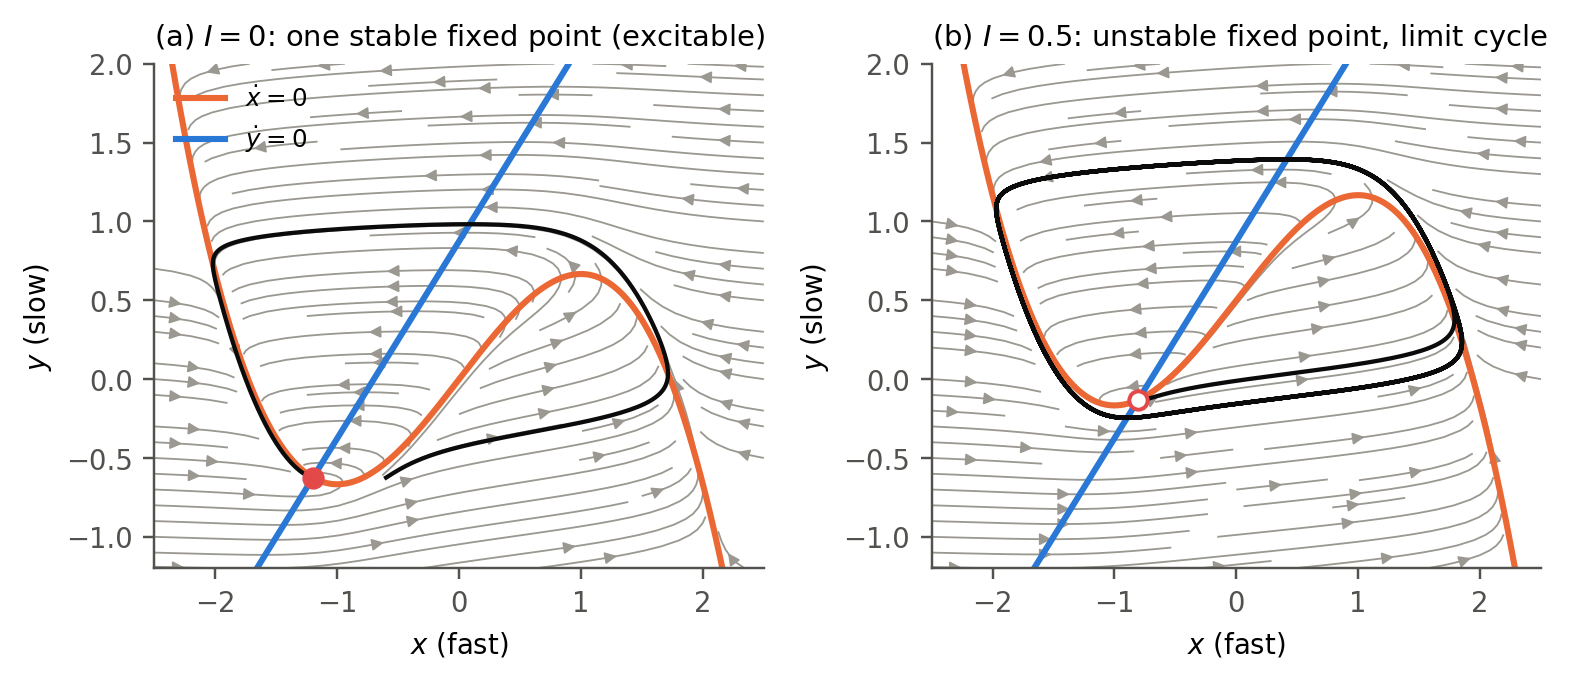
\includegraphics[width=0.95\linewidth]{f03_nullclines.png}
\caption{FitzHugh--Nagumo. Orange: $x$-nullcline; blue: $y$-nullcline; black: one trajectory. (a) At $I=0$ the fixed
point lies on the left (attracting) part of the cubic: stable. A kick large enough to cross the middle branch produces one
large excursion (a spike) before returning: \emph{excitability}. (b) At $I=0.5$ the fixed point is on the middle branch:
unstable, and every trajectory converges to a limit cycle.}\label{fig:nc}
\end{figure}

\begin{worked}[Stability of the FitzHugh--Nagumo fixed point]
$J = \begin{pmatrix} 1 - x^{*2} & -1\\ \eps & -\eps b\end{pmatrix}$, so
$\tau = 1 - x^{*2} - \eps b$ and $\Delta = \eps\,[1 - b(1 - x^{*2})]$.
\begin{itemize}
\item $\Delta>0$ as long as $1 - x^{*2} < 1/b = 1.25$, which always holds: no saddle-node here.
\item $\tau = 0$ when $x^{*2} = 1 - \eps b = 0.936$, i.e.\ $x^* = -0.9675$. The fixed point solves
$I = (x^*+a)/b - x^* + x^{*3}/3$, which gives $I_H = 0.3313$. Below $I_H$, $\tau<0$ (stable); above, $\tau>0$ (unstable).
\end{itemize}
The fixed point therefore loses stability through a Hopf bifurcation at $I_H = 0.3313$, close to where it reaches the
minimum (the ``knee'') of the cubic. Its frequency there is $\omega = \sqrt\Delta = 0.276$. Whether the Hopf is
supercritical or subcritical needs one more number (Chapter 5): here it is subcritical.
\end{worked}

\section{Limit cycles and the Poincaré--Bendixson theorem}\label{sec:pb}
A \textbf{limit cycle} is an isolated closed trajectory. It is stable if neighbouring trajectories spiral onto it, and
unstable if they spiral away. In two dimensions there is a powerful existence result.

\begin{keyidea}[Poincaré--Bendixson]
If a bounded region of the plane traps trajectories (the flow on its boundary points inwards) and contains no fixed
point, or only unstable foci or nodes, then it contains a limit cycle. In particular, in two dimensions a bounded
trajectory ends up either at a fixed point or on a closed orbit: \emph{there is no chaos in the plane.}
\end{keyidea}
In Fig.~\ref{fig:nc}b, a large box around the cubic traps the flow and the only fixed point inside is unstable, so a
limit cycle must exist. A useful companion is the \emph{Bendixson criterion}: if $\partial_x f + \partial_y g$ has one
sign in a simply connected region, that region contains no closed orbit.

%==========================================================================================
\chapter{Saddle-node, transcritical and pitchfork bifurcations}
%==========================================================================================
A \textbf{bifurcation} is a parameter value at which the phase portrait changes qualitatively: fixed points or cycles
appear, disappear or change stability. Away from bifurcations, small parameter changes only deform the portrait.

\section{The saddle-node (fold) bifurcation}
The normal form is
\[
\dot x = \mu + x^2 .
\]
\begin{itemize}
\item $\mu<0$: two fixed points $x^* = \pm\sqrt{-\mu}$. Since $f'(x^*) = 2x^*$, the lower one is stable and the upper one
unstable.
\item $\mu=0$: they merge into one half-stable point at $x=0$, with $f'(0)=0$.
\item $\mu>0$: no fixed point; $x$ runs away.
\end{itemize}
In two dimensions, adding a stable direction ($\dot y = -y$) turns the stable point into a stable \emph{node} and the
unstable one into a \emph{saddle}: the bifurcation is a collision of a node with a saddle, hence its name
(Fig.~\ref{fig:sn}). The word \textbf{fold} refers to the bifurcation diagram: the branch of fixed points $\mu = -x^2$ is
a parabola that folds back at $\mu=0$. ``Saddle-node'', ``fold'' and ``limit point'' are the same thing.

\begin{figure}[H]\centering
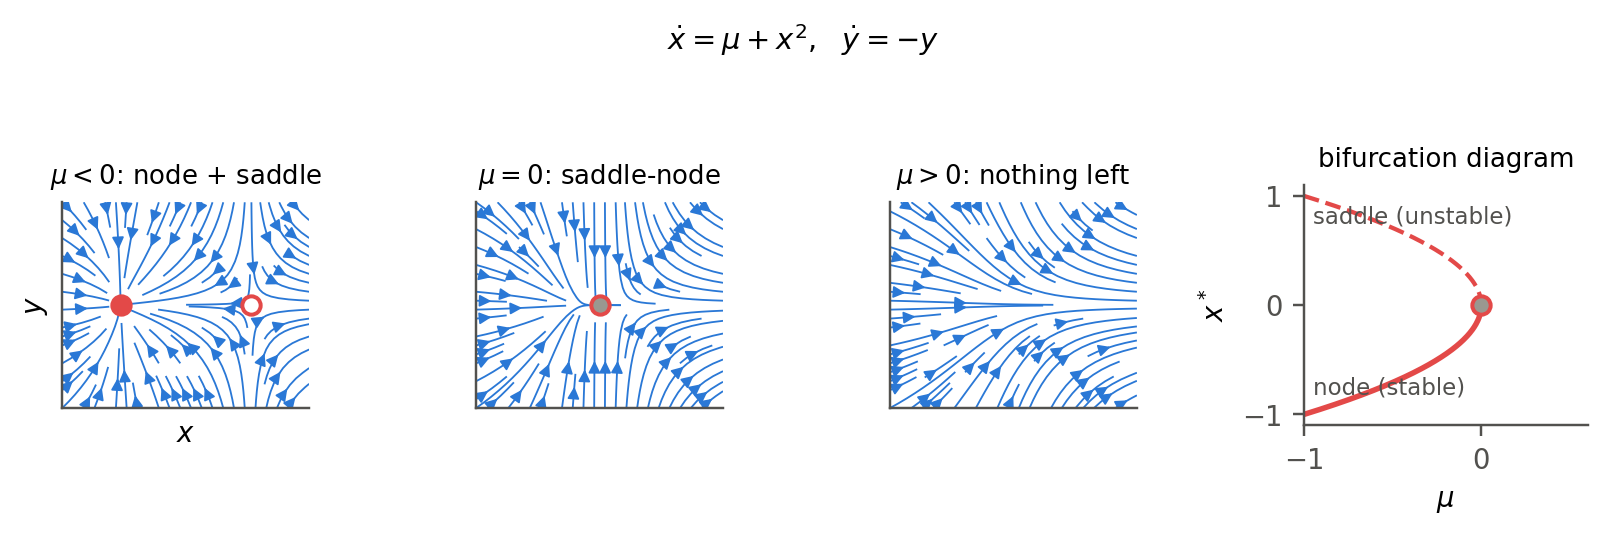
\includegraphics[width=\linewidth]{f04_saddlenode.png}
\caption{Saddle-node bifurcation. A node and a saddle approach, merge, and disappear. Right: the fold in the
bifurcation diagram.}\label{fig:sn}
\end{figure}

\begin{keyidea}[{Conditions for a saddle-node, in any dimension}]
At $(x^*,\mu_c)$: (i) $f(x^*,\mu_c) = 0$; (ii) the Jacobian has a single zero eigenvalue ($\Delta=0$ in 2D), i.e.\ in 1D
$f_x = 0$; (iii) nondegeneracy, $f_{xx} \ne 0$ (the branch really folds); (iv) transversality, $f_\mu\ne0$ (the
parameter really unfolds it). Under these conditions the system near the fold is equivalent to $\dot x = \mu + x^2$.
\end{keyidea}

\textbf{Two fingerprints.}
\begin{enumerate}
\item \textbf{Square-root law.} The two fixed points are separated by $2\sqrt{\mu_c - \mu}$, and their eigenvalues are
$\pm 2\sqrt{\mu_c-\mu}$: both go to zero at the fold. Near the fold, the stable state relaxes ever more slowly
(\emph{critical slowing down}).
\item \textbf{Ghost and bottleneck.} Just past the fold ($\mu$ small and positive), there is no fixed point, but the flow
is still very slow near $x=0$. The time to get through is
\[
T = \int_{-\infty}^{\infty}\frac{dx}{\mu + x^2} = \frac{\pi}{\sqrt{\mu}}\ \to\infty\ \text{ as }\mu\to0^+ .
\]
The vanished fixed point leaves a \emph{ghost}. This $1/\sqrt\mu$ law is the signature of the SNIC (Chapter 6).
\end{enumerate}

\begin{keyidea}[{A ball in honey: picturing a fold}]
Any one-variable flow $\dot x = f(x)$ is a ball rolling on the landscape $V(x) = -\int f\,dx$ (\S1.3), with two rules: it
always rolls downhill, and it moves in honey (no inertia: it stops as soon as the ground is flat). Valleys are stable
fixed points, hilltops unstable ones. For $\dot x = \mu + x^2$, $V = -\mu x - x^3/3$ (Fig.~\ref{fig:land}, top):
\begin{itemize}
\item $\mu<0$: a valley (the ball rests) next to a hilltop (the threshold: kicked over it, the ball rolls away);
\item $\mu\to0^-$: the valley gets shallower and the hilltop lower; after a kick the ball wobbles back ever more slowly
(critical slowing down), and a small push gets it over;
\item $\mu=0$: valley and hilltop merge into a flat ledge: the fold;
\item $\mu>0$: only a slope with an almost flat shelf where the valley was (the ghost); the ball rolls off, crawling over
the shelf first (the bottleneck time $\pi/\sqrt\mu$).
\end{itemize}
A saddle-node is a valley disappearing under the ball.
\end{keyidea}

\begin{figure}[H]\centering
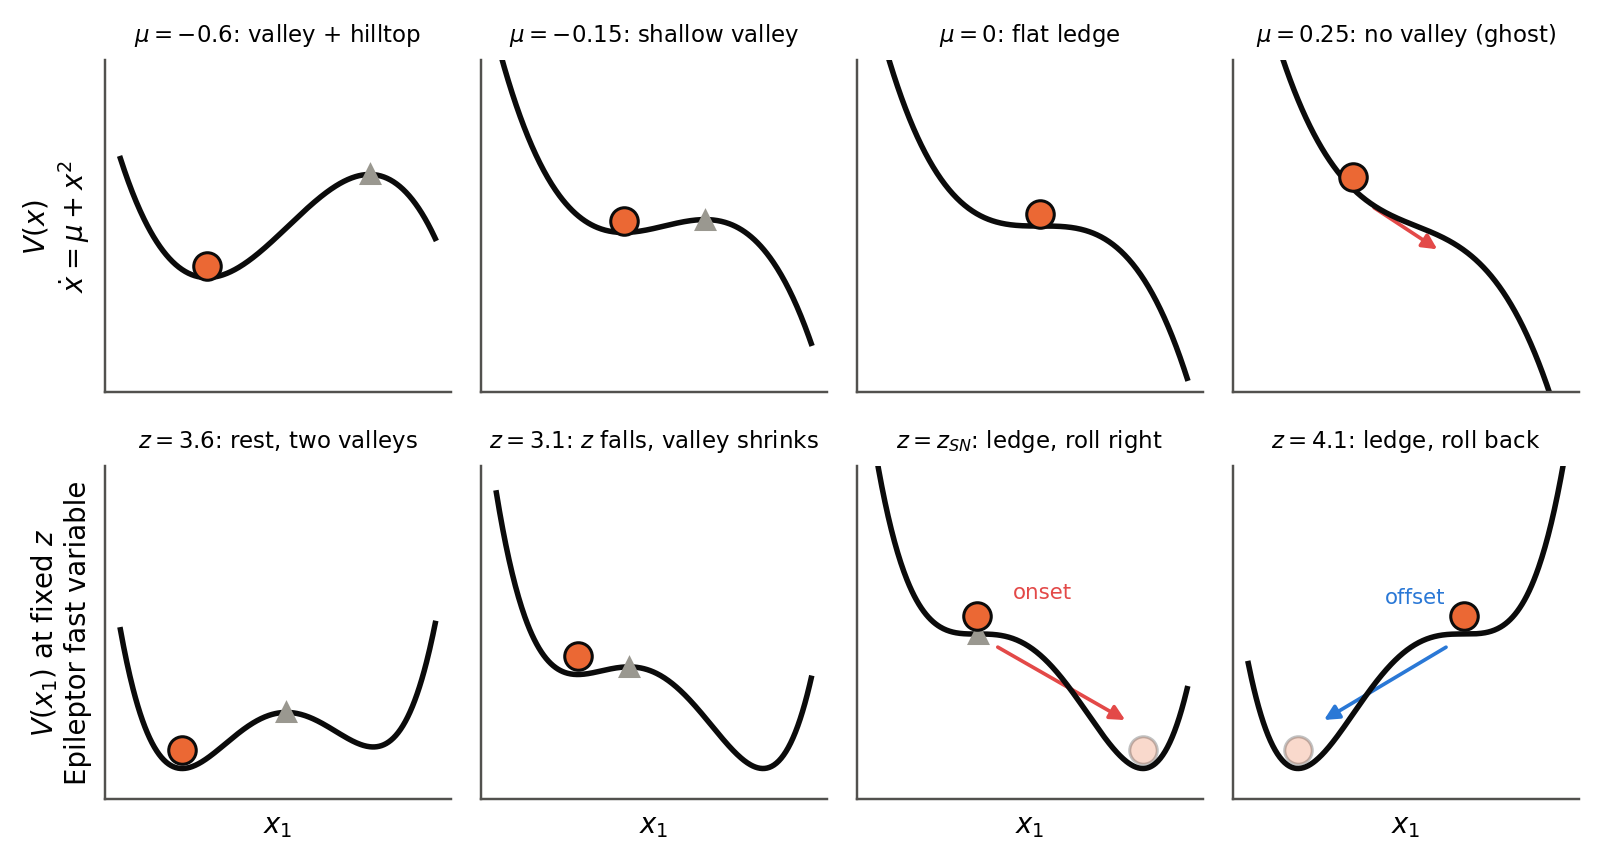
\includegraphics[width=\linewidth]{f12_landscape.png}
\caption{Bottom row: the same picture for the Epileptor's fast variable at fixed $z$,
$V(x_1) = x_1^4/4 + 2x_1^3/3 - (1+I_{ext}-z)\,x_1$, a double well (left valley: rest; right valley: seizure; grey
triangle: the crest between them, the repelling branch). The slow variable $z$ tilts the board. As $z$ falls the left
valley shrinks; at $z=z_{SN}$ it becomes a ledge and the ball rolls into the right valley (onset); during the seizure $z$
rises and tilts the board back until, at $z=4.1$, the right valley disappears and the ball rolls back (offset).
Chapter 11 uses this picture.}\label{fig:land}
\end{figure}

\section{Transcritical and pitchfork bifurcations}
These need a special structure, so they are not generic, but they are common in models with a fixed point that
always exists (for example a zero population) or with a symmetry $x\to-x$ (Fig.~\ref{fig:tp}).
\begin{itemize}
\item \textbf{Transcritical}, $\dot x = \mu x - x^2$: the fixed points $0$ and $\mu$ cross and exchange stability.
\item \textbf{Supercritical pitchfork}, $\dot x = \mu x - x^3$: for $\mu>0$ the origin becomes unstable and two symmetric
stable states $\pm\sqrt\mu$ appear, growing continuously from zero.
\item \textbf{Subcritical pitchfork}, $\dot x = \mu x + x^3$: the two side branches are unstable and exist for $\mu<0$; at
$\mu=0$ the origin loses stability with nothing nearby to go to, so the state jumps far away. Adding a $-x^5$ term
creates large stable branches and hysteresis (compare the subcritical Hopf, \S\ref{sec:subhopf}).
\end{itemize}

\begin{figure}[H]\centering
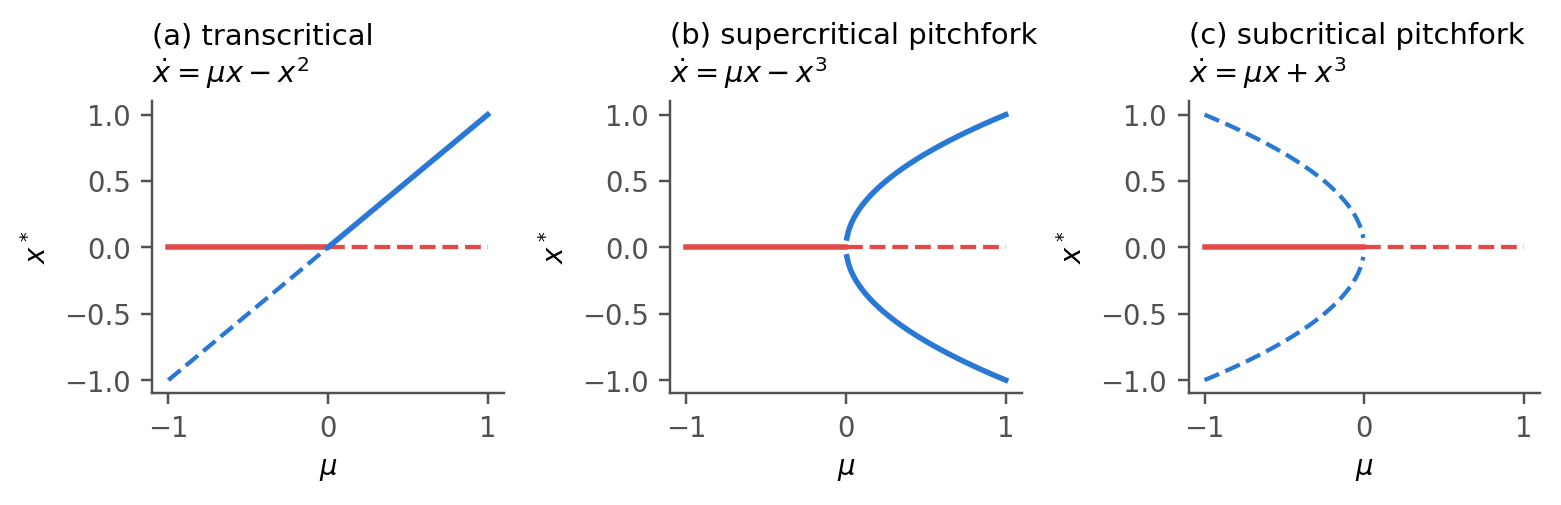
\includegraphics[width=\linewidth]{f05_trans_pitch.png}
\caption{Transcritical and pitchfork bifurcations (solid: stable; dashed: unstable).}\label{fig:tp}
\end{figure}

\subsection*{The math behind Fig.~\ref{fig:tp}}
Each panel is drawn with the same three steps as any one-dimensional bifurcation diagram:
\begin{enumerate}
\item solve $f(x,\mu)=0$ for the fixed points $x^*(\mu)$ and plot them against $\mu$;
\item compute the eigenvalue $\lambda = \partial_x f(x^*,\mu)$ on each branch (Chapter 1);
\item draw the branch solid where $\lambda<0$ (stable) and dashed where $\lambda>0$ (unstable).
\end{enumerate}

\begin{worked}[(a) Transcritical: $\dot x = \mu x - x^2$]
\textbf{Fixed points.} Factor: $f = x(\mu - x) = 0$, so $x^* = 0$ or $x^* = \mu$. Both exist for every $\mu$: in the
diagram, the horizontal line $x^*=0$ and the diagonal $x^* = \mu$.

\textbf{Eigenvalue.} $\partial_x f = \mu - 2x$.
\begin{itemize}
\item On $x^* = 0$: $\lambda = \mu$. Stable for $\mu<0$, unstable for $\mu>0$.
\item On $x^* = \mu$: $\lambda = \mu - 2\mu = -\mu$. Unstable for $\mu<0$, stable for $\mu>0$.
\end{itemize}
\textbf{At $\mu = 0$} the two branches cross at $x=0$ and both eigenvalues are zero; on either side the two fixed points
have swapped stability. That is why the line $x^*=0$ is solid on the left and dashed on the right, and the diagonal the
opposite.

\textbf{Why it is not a saddle-node.} The saddle-node conditions of \S4.1 include transversality, $\partial_\mu f\ne0$.
Here $\partial_\mu f = x$, which is $0$ at the bifurcation point. This is the structural reason: the factor $x$ forces
$x=0$ to stay a fixed point for every $\mu$, so the branches cannot fold and vanish; they can only cross.
\end{worked}

\begin{worked}[(b) Supercritical pitchfork: $\dot x = \mu x - x^3$]
\textbf{Fixed points.} $f = x(\mu - x^2) = 0$: $x^* = 0$ for every $\mu$, and $x^{*2} = \mu$, i.e.\ $x^* = \pm\sqrt\mu$, which
exists only for $\mu>0$. In the diagram the side branches form the parabola $\mu = x^2$, opening to the right.

\textbf{Eigenvalue.} $\partial_x f = \mu - 3x^2$.
\begin{itemize}
\item On $x^* = 0$: $\lambda = \mu$. Stable for $\mu<0$, unstable for $\mu>0$.
\item On $x^* = \pm\sqrt\mu$ ($\mu>0$): $\lambda = \mu - 3\mu = -2\mu < 0$. Both side branches are stable.
\end{itemize}
\textbf{Reading.} As $\mu$ crosses 0, the origin loses stability and hands it to two new stable states that start at
$x=0$ and grow as $\sqrt\mu$: a smooth, reversible transition (supercritical). The relaxation rate near the origin,
$|\lambda| = |\mu|$, goes to zero at the bifurcation: critical slowing down.

\textbf{Why three branches.} $f(-x,\mu) = -f(x,\mu)$: the equation is unchanged by $x\to-x$, so if $x^*$ is a fixed point
so is $-x^*$. The symmetry forces the side branches to come in pairs.
\end{worked}

\begin{worked}[(c) Subcritical pitchfork: $\dot x = \mu x + x^3$]
\textbf{Fixed points.} $f = x(\mu + x^2) = 0$: $x^* = 0$, and $x^{*2} = -\mu$, i.e.\ $x^* = \pm\sqrt{-\mu}$, which exists only
for $\mu<0$. The side branches form the parabola $\mu = -x^2$, opening to the \emph{left}.

\textbf{Eigenvalue.} $\partial_x f = \mu + 3x^2$.
\begin{itemize}
\item On $x^* = 0$: $\lambda = \mu$, as before.
\item On $x^* = \pm\sqrt{-\mu}$ ($\mu<0$): $\lambda = \mu + 3(-\mu) = -2\mu > 0$. Both side branches are unstable.
\end{itemize}
\textbf{Reading.} For $\mu<0$ the stable origin is flanked by two unstable states at $\pm\sqrt{-\mu}$; they are thresholds:
a perturbation larger than $\sqrt{-\mu}$ escapes. As $\mu\to0^-$ the thresholds close in on the origin, and at $\mu=0$ the
origin becomes unstable with no stable state nearby: the state runs away (here to infinity). This is the subcritical
case.
\end{worked}

\begin{worked}[(d) Adding $-x^5$: where hysteresis comes from]
$\dot x = \mu x + x^3 - x^5$. Besides $x^*=0$, the fixed points solve $\mu + x^2 - x^4 = 0$, a quadratic in $s = x^2$:
\[
s^2 - s - \mu = 0\quad\Rightarrow\quad x^{*2} = s_\pm = \frac{1\pm\sqrt{1+4\mu}}{2}.
\]
\begin{itemize}
\item $s_+$ exists for $\mu\ge-1/4$; $s_-$ is positive only for $-1/4<\mu<0$. They merge at $\mu = -1/4$, $x^{*2} = 1/2$:
a \textbf{saddle-node (fold)} of the side branches.
\item Stability: on a branch, $\mu = x^4 - x^2$, so
$\partial_x f = \mu + 3x^2 - 5x^4 = (x^4 - x^2) + 3x^2 - 5x^4 = 2x^2(1 - 2x^2)$.
It is positive (unstable) for $x^{*2}<1/2$ (the inner branch $s_-$) and negative (stable) for $x^{*2}>1/2$ (the outer
branch $s_+$).
\end{itemize}
So for $-1/4<\mu<0$ there are three stable states (0 and $\pm\sqrt{s_+}$) separated by the two unstable ones: bistability.
Increasing $\mu$ past 0, the state jumps from 0 to the outer branch; decreasing it, it stays on the outer branch down to
the fold at $\mu=-1/4$, then falls back to 0. This is exactly the radius equation of the subcritical Hopf in Chapter 5
($\dot r = \mu r + r^3 - r^5$, fold of cycles at $\mu=-1/4$, $r^2 = 1/2$), and the hysteresis loop of Chapter 7.
\end{worked}

\begin{keyidea}[{Super- versus subcritical}]
This distinction recurs everywhere. \textbf{Supercritical}: the new stable state is born \emph{at} the old one and grows
continuously, so the transition is smooth and reversible. \textbf{Subcritical}: the new state branches \emph{backwards}
and is unstable, so when the old state loses stability the system jumps to a distant state, and it does not come back
at the same parameter value (hysteresis).
\end{keyidea}

%==========================================================================================
\chapter{Hopf bifurcations}
%==========================================================================================
\section{The normal form}
A Hopf bifurcation happens when a stable focus becomes unstable, i.e.\ when a complex pair of eigenvalues
$\lambda = \mu\pm i\omega$ crosses the imaginary axis ($\tau$ crosses 0 with $\Delta>0$). In polar coordinates
$(r,\theta)$, the normal form is
\[
\dot r = \mu\,r + \ell_1\,r^3,\qquad \dot\theta = \omega + \dots
\]
The angle just rotates; the radius obeys a one-dimensional equation that is exactly the pitchfork of the last chapter. A
fixed point $r^*>0$ of the radius equation is a circle in the plane: a \textbf{limit cycle} of radius $r^*$. The sign of
the \textbf{first Lyapunov coefficient} $\ell_1$ decides the type.

\section{Supercritical Hopf ($\ell_1<0$)}
With $\ell_1 = -1$: for $\mu<0$ the origin is a stable focus; for $\mu>0$ it is unstable and surrounded by a stable
limit cycle of radius $\sqrt\mu$ (Fig.~\ref{fig:hopf}, top). The oscillation is born with zero amplitude and grows as the
square root of the distance to the bifurcation, at a finite frequency $\omega$. The transition is smooth and reversible.

\section{Subcritical Hopf ($\ell_1>0$)}\label{sec:subhopf}
With $\ell_1>0$ the small cycle exists for $\mu<0$ and is \emph{unstable}. A higher-order term ($-r^5$) usually provides
a large stable cycle, and the two cycles merge and disappear in a \textbf{fold of limit cycles} (saddle-node of cycles)
at some $\mu_f<0$. With $\dot r = \mu r + r^3 - r^5$ (Fig.~\ref{fig:hopf}, bottom):
\begin{itemize}
\item $\mu<-1/4$: only the stable focus.
\item $-1/4<\mu<0$: \textbf{bistability}. The stable focus is surrounded by an unstable cycle (the threshold), which is
surrounded by a stable large cycle. Small perturbations decay; large ones jump to the big oscillation.
\item $\mu>0$: the focus is unstable, and the system jumps to the large cycle, whose amplitude is finite immediately.
\end{itemize}
Coming back down, the large oscillation persists until $\mu = -1/4$: hysteresis (Chapter 7).

\begin{figure}[H]\centering
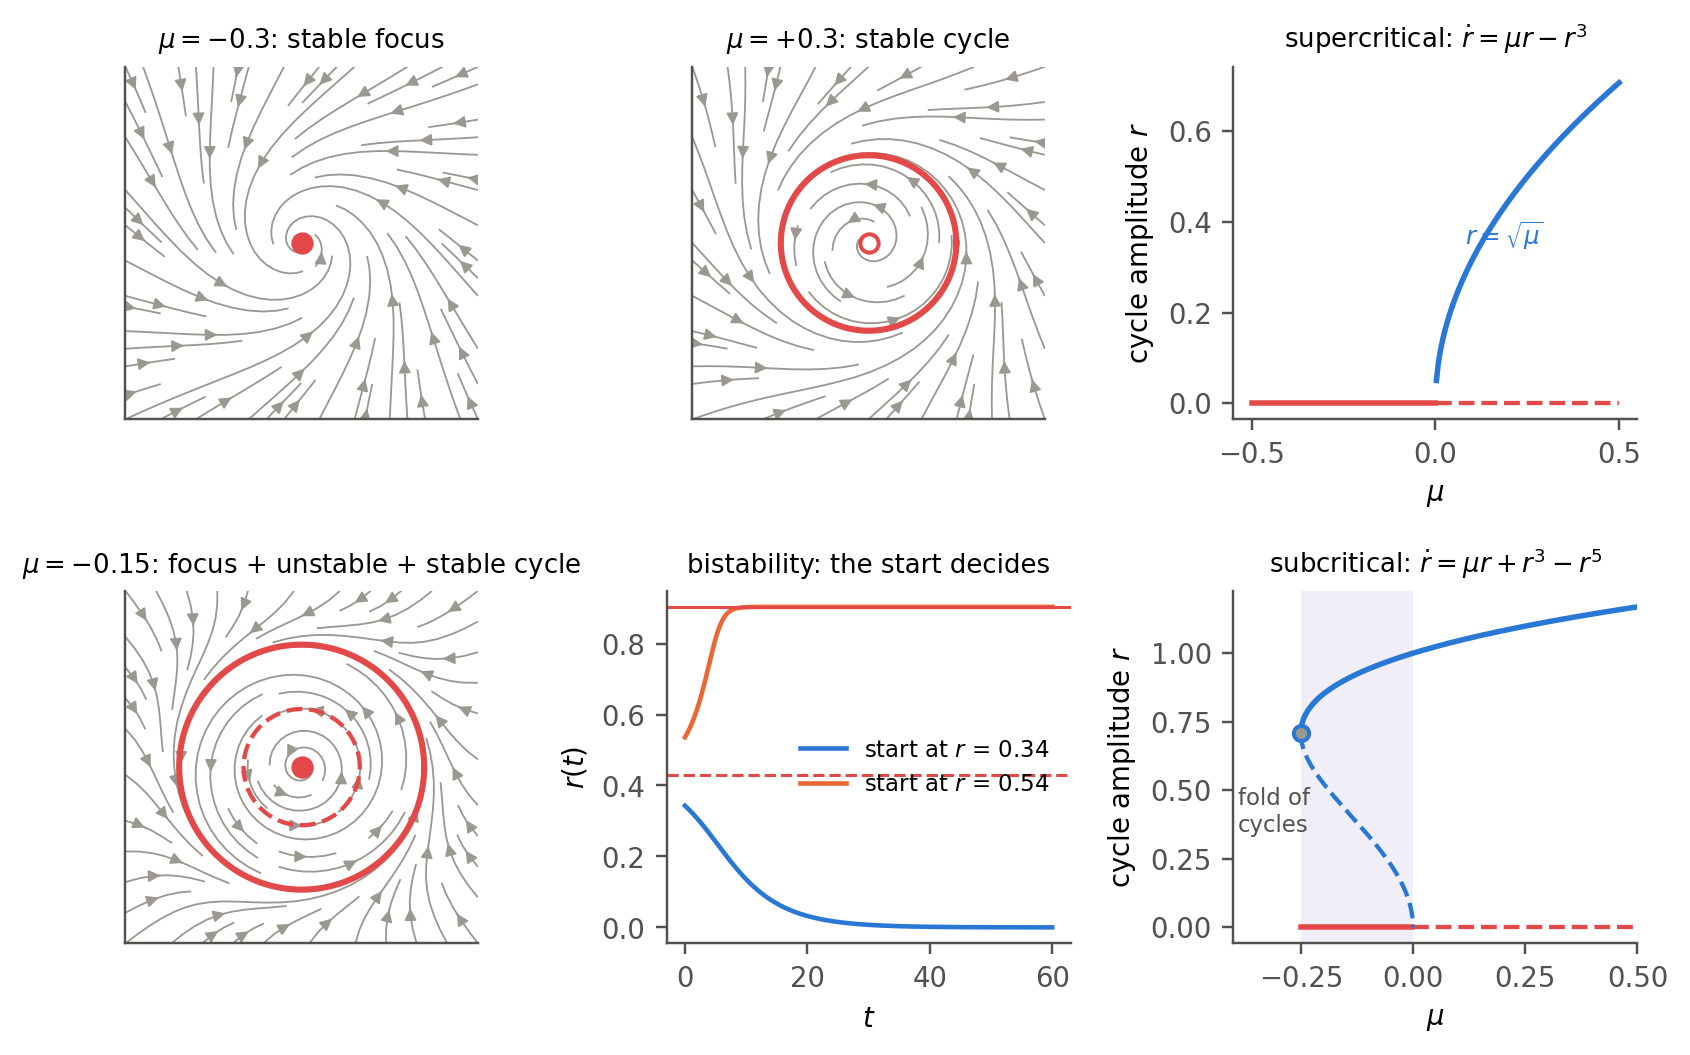
\includegraphics[width=\linewidth]{f06_hopf.png}
\caption{Top: supercritical Hopf. Bottom: subcritical Hopf with a fold of cycles at $\mu=-1/4$; in the shaded window,
rest and oscillation coexist, separated by the unstable cycle (dashed).}\label{fig:hopf}
\end{figure}

\section{Deciding super or sub from the equations}
Bring the system to the form where the fixed point is at the origin and the linear part at the bifurcation is a pure
rotation,
\[
\dot u = -\omega v + F(u,v),\qquad \dot v = \omega u + G(u,v),
\]
where $F$, $G$ contain the nonlinear terms (in general this needs a linear change of coordinates built from the real and
imaginary parts of the eigenvector). Then \cite{guckenheimer}
\[
\ell_1 = \tfrac{1}{16}\big[F_{uuu} + F_{uvv} + G_{uuv} + G_{vvv}\big]
+ \tfrac{1}{16\,\omega}\big[F_{uv}(F_{uu}+F_{vv}) - G_{uv}(G_{uu}+G_{vv}) - F_{uu}G_{uu} + F_{vv}G_{vv}\big],
\]
all derivatives at the origin. $\ell_1<0$: supercritical; $\ell_1>0$: subcritical.

\begin{worked}[{Checking the formula, then FitzHugh--Nagumo}]
\textbf{Check.} $F = -u(u^2+v^2)$, $G = -v(u^2+v^2)$ (the supercritical normal form). $F_{uuu} = -6$, $F_{uvv} = -2$,
$G_{uuv}=-2$, $G_{vvv}=-6$, and all second derivatives vanish, so $\ell_1 = -16/16 = -1$: supercritical, as it should be.

\textbf{FitzHugh--Nagumo at $I_H = 0.3313$.} Shifting the fixed point to the origin and rotating into the eigenvector
basis gives a pure rotation with $\omega = 0.2755$, and the formula gives $\ell_1 = +0.067$: \emph{subcritical}. A
simulation confirms it: at $I = 0.325 < I_H$, a trajectory started far away settles on a large cycle (amplitude 3.7),
while the fixed point is still stable; at $I = 0.30$ only the fixed point remains. The amplitude just above $I_H$ is
already 3.76, not small.
\end{worked}

\begin{recipe}[Super or sub without the formula]
Simulate just past the bifurcation and look at the amplitude: small and growing like $\sqrt{\mu-\mu_c}$ means
supercritical; large immediately means subcritical. Then simulate just before it from a large initial condition: if a
large oscillation survives, the system is bistable, confirming subcritical.
\end{recipe}

\begin{pitfall}
In slow--fast systems (Chapter 8), a Hopf bifurcation can be supercritical and yet look abrupt: the small cycle grows
into a large relaxation oscillation over an exponentially small parameter range (a \emph{canard explosion}). The
amplitude test above then needs a very fine parameter scan.
\end{pitfall}

%==========================================================================================
\chapter{Global bifurcations of limit cycles}
%==========================================================================================
Local bifurcations are decided by the Jacobian at a fixed point. Global ones involve a whole cycle and cannot be found
by linearisation. Three matter here.

\section{Saddle-node on invariant circle (SNIC)}
Consider $\dot r = r(1-r^2)$, $\dot\theta = \omega - \sin\theta$. The circle $r=1$ attracts everything. On it, the angle
obeys a one-dimensional equation (Fig.~\ref{fig:snic}):
\begin{itemize}
\item $\omega<1$: $\sin\theta^* = \omega$ has two solutions on the circle, a node and a saddle. The circle is made of the
two connections between them; the state rests at the node.
\item $\omega = 1$: they merge in a saddle-node \emph{on} the circle.
\item $\omega>1$: no fixed point is left; the state goes round the circle forever: a limit cycle.
\end{itemize}
The oscillation is born with finite amplitude (the size of the circle) but \emph{zero frequency}: the state spends a
very long time in the bottleneck left by the ghost. The period is
\[
T = \int_0^{2\pi}\frac{d\theta}{\omega - \sin\theta} = \frac{2\pi}{\sqrt{\omega^2-1}} \sim \frac{\pi\sqrt2}{\sqrt{\omega-1}} .
\]
A saddle-node that happens on a closed loop is a SNIC; one that happens elsewhere just destroys a rest state, and the
system jumps to whatever else is there (another fixed point or an existing cycle).

\begin{figure}[H]\centering
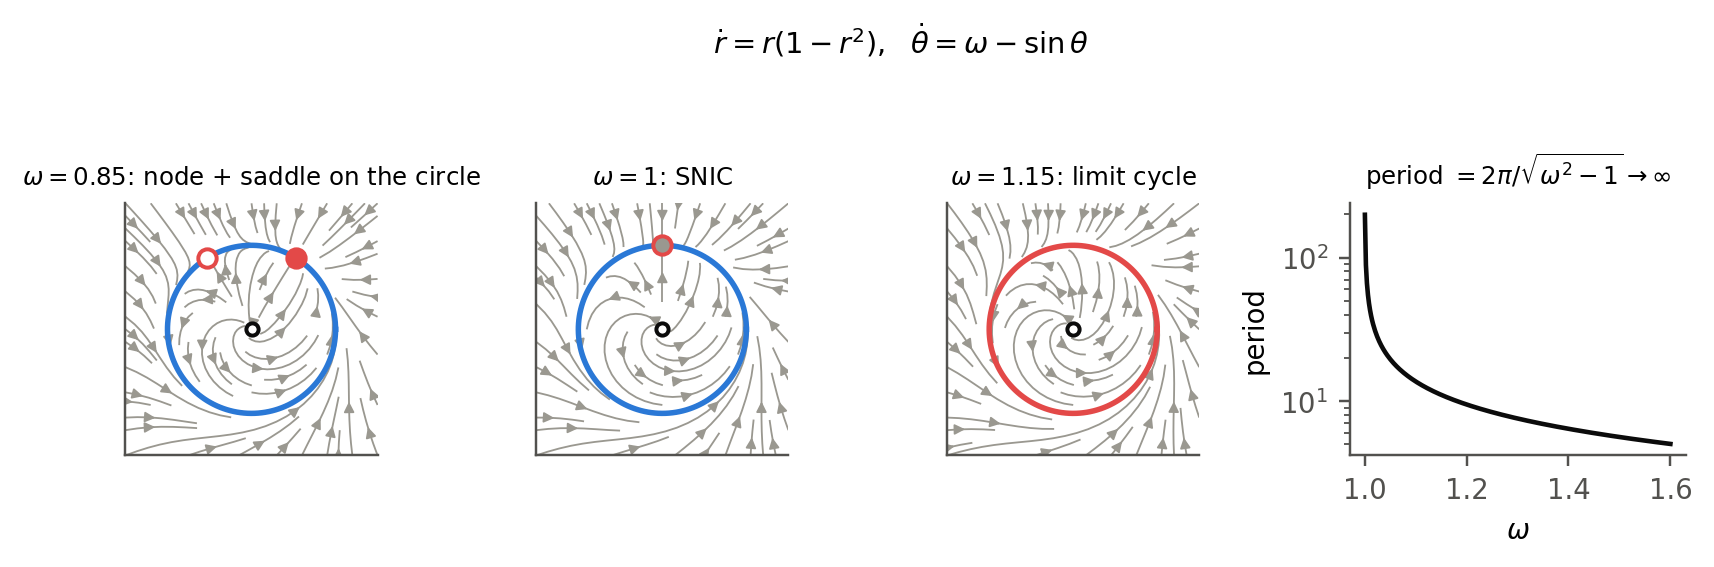
\includegraphics[width=\linewidth]{f07_snic.png}
\caption{SNIC: node and saddle merge on the invariant circle, leaving a periodic orbit whose period diverges as
$1/\sqrt{\omega-1}$.}\label{fig:snic}
\end{figure}

\section{Homoclinic (saddle-loop) bifurcation}
A limit cycle grows until it touches a saddle. At that moment it becomes a \textbf{homoclinic orbit}: a trajectory
that leaves the saddle along its unstable manifold and comes back along its stable manifold. Past the bifurcation the
loop breaks and the cycle is gone.

The example of Fig.~\ref{fig:homo} is $\dot x = y$, $\dot y = \mu y + x - x^2 + xy$, with a saddle at $(0,0)$ and a
focus at $(1,0)$. A stable cycle is born from the focus by a supercritical Hopf at $\mu=-1$; as $\mu$ increases it grows,
touches the saddle at $\mu_c\approx-0.8645$, and disappears.

\textbf{Fingerprint.} Near the saddle the flow is slow, and the cycle passes ever closer to it: the time spent there
grows like $-\ln(\text{distance})/\lambda_u$, where $\lambda_u$ is the saddle's unstable eigenvalue. So the period grows
\emph{logarithmically}, $T\sim -\lambda_u^{-1}\ln|\mu-\mu_c|$ (a straight line on a semilog plot, Fig.~\ref{fig:homo},
right), while the amplitude stays finite. Compare the SNIC: there the period grows as $1/\sqrt{|\mu-\mu_c|}$, much faster.

\begin{figure}[H]\centering
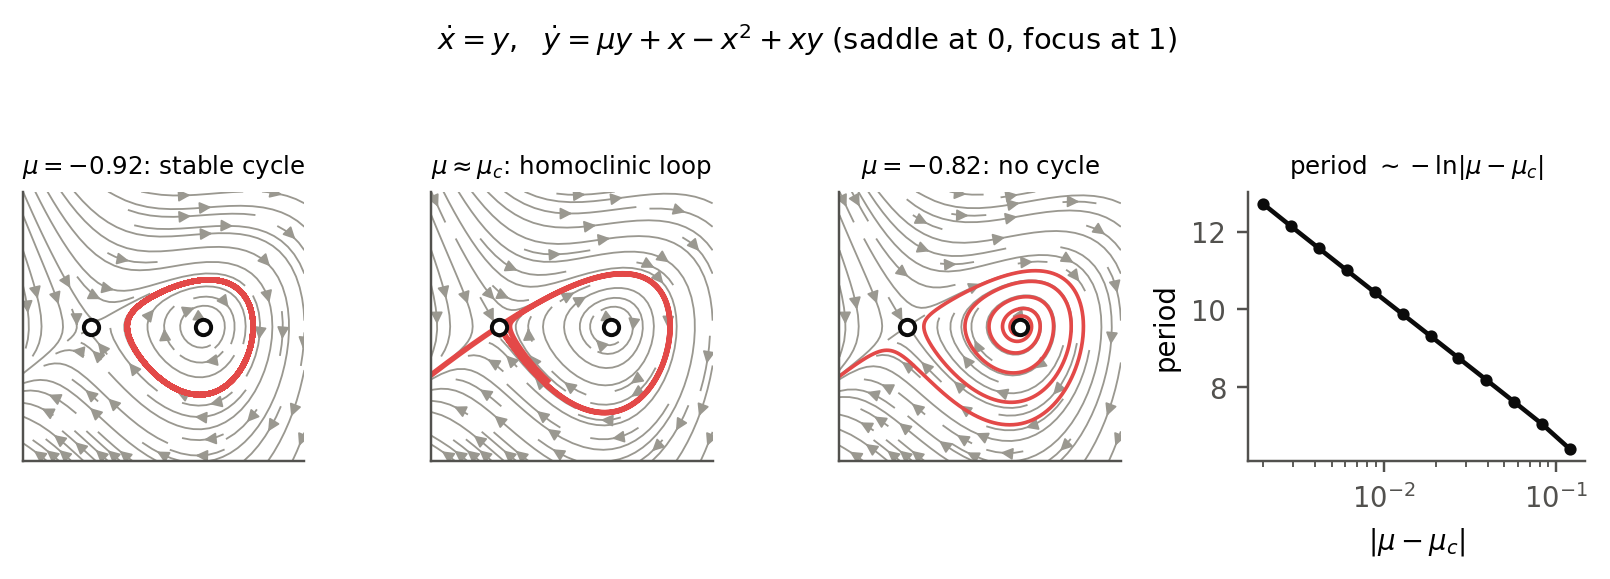
\includegraphics[width=\linewidth]{f08_homoclinic.png}
\caption{Homoclinic bifurcation. The stable cycle (red) grows, touches the saddle, and disappears; afterwards
trajectories spiral out of the unstable focus and escape. Right: the period diverges logarithmically.}\label{fig:homo}
\end{figure}

\section{Fold of limit cycles}
A stable and an unstable cycle merge and disappear (the bottom right of Fig.~\ref{fig:hopf}, at $\mu=-1/4$). Nothing
special happens to the period or the amplitude of the stable cycle as it approaches the fold: both stay finite. The
oscillation simply stops, and the system falls to whatever attractor is left (usually a stable fixed point).

\section{How oscillations start and stop: the four onsets and four offsets}
For a neuron, a seizure or any system going from rest to oscillation, there are four generic ways for the oscillation to
appear and four generic ways for it to end \cite{izhikevich}. They can be told apart from recordings.

\begin{center}\small
\begin{tabular}{>{\raggedright}p{3.3cm}>{\raggedright}p{2.7cm}>{\raggedright}p{2.6cm}p{5.6cm}}
\toprule
bifurcation & amplitude at onset & frequency at onset & what the rest state does \\
\midrule
\multicolumn{4}{l}{\textbf{Onset} (rest $\to$ oscillation)}\\
saddle-node (off cycle) & finite, jump & finite & rest disappears; jump to a coexisting cycle; baseline shift \\
SNIC & finite & $\to0$ as $\sqrt{\mu-\mu_c}$ & rest disappears on the future cycle \\
supercritical Hopf & $\to0$ as $\sqrt{\mu-\mu_c}$ & finite ($\omega$) & rest becomes an unstable focus \\
subcritical Hopf & finite, jump & finite & rest becomes unstable; bistability before \\
\midrule
\multicolumn{4}{l}{\textbf{Offset} (oscillation $\to$ rest)}\\
saddle-homoclinic & finite & $\to0$ as $1/|\ln(\mu-\mu_c)|$ & cycle hits a saddle \\
SNIC & finite & $\to0$ as $\sqrt{\mu-\mu_c}$ & node and saddle reappear on the cycle \\
supercritical Hopf & $\to0$ & finite & cycle shrinks onto the focus \\
fold of limit cycles & finite & finite & cycle merges with an unstable one \\
\bottomrule
\end{tabular}
\end{center}

\begin{keyidea}[Reading a recording]
Does the oscillation start small and grow? Supercritical Hopf. Does it start large? Then look at the frequency: slow at
first (and speeding up) means SNIC; fast immediately means saddle-node or subcritical Hopf, which the presence of a
baseline (DC) shift and bistability help separate. At the end: does the frequency slow down before stopping while the
amplitude stays large? Homoclinic (logarithmic) or SNIC (square-root). Does the amplitude shrink? Supercritical Hopf.
\end{keyidea}

%==========================================================================================
\chapter{Bistability and hysteresis}
%==========================================================================================
\section{Two folds make a hysteresis loop}
Take $\dot x = \mu + x - x^3$. The fixed points satisfy $\mu = x^3 - x$, an S-shaped curve (Fig.~\ref{fig:hyst}a). It
has two folds where $d\mu/dx = 3x^2 - 1 = 0$, at $x = \pm1/\sqrt3$, $\mu = \mp2/(3\sqrt3) = \mp0.385$. Between them,
three fixed points coexist: two stable branches (upper and lower) and an unstable middle branch. Now let $\mu$ change
slowly:
\begin{enumerate}
\item Starting on the lower branch and increasing $\mu$, the state follows the lower branch until it ends at the fold
$\mu = +0.385$. There the stable state disappears in a saddle-node and the state \textbf{jumps up} to the upper branch.
\item Decreasing $\mu$ again, the state follows the upper branch, past the point where it jumped up, down to the other
fold at $\mu=-0.385$, where it \textbf{jumps down}.
\end{enumerate}
The path traced is a loop: the state at a given $\mu$ depends on where it came from. This is \textbf{hysteresis}: memory
of the history, caused by \textbf{bistability} (two stable states for the same parameter) between two folds.

\begin{figure}[H]\centering
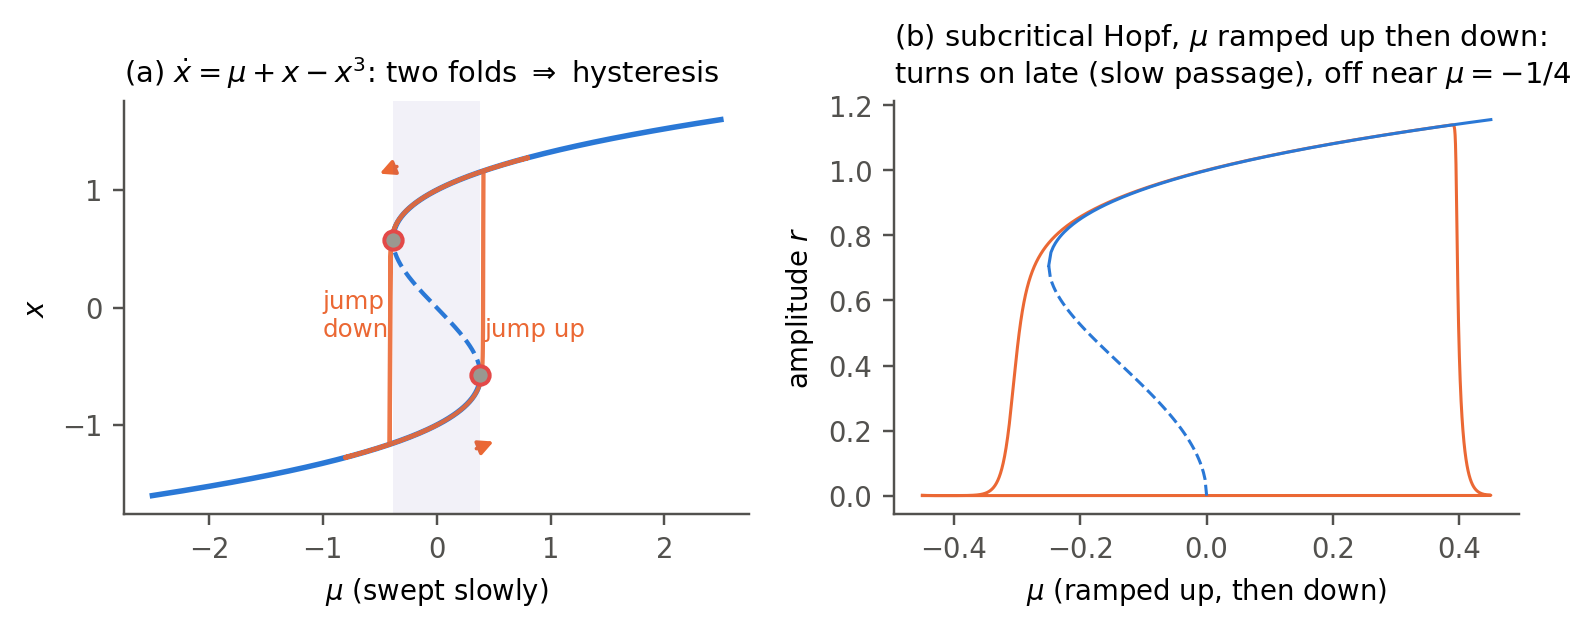
\includegraphics[width=\linewidth]{f09_hysteresis.png}
\caption{(a) Hysteresis between two saddle-node bifurcations: an S-shaped branch of fixed points and a slow sweep of
$\mu$ (orange). (b) Hysteresis at a subcritical Hopf: the oscillation turns on late on the way up and stays on below
$\mu = 0$ on the way down.}\label{fig:hyst}
\end{figure}

\section{Hysteresis with oscillations}
At a subcritical Hopf with a fold of cycles (Fig.~\ref{fig:hyst}b), the same thing happens between a rest state and an
oscillation: increasing the parameter, the oscillation starts at the Hopf ($\mu=0$); decreasing it, it stops only at
the fold of cycles ($\mu = -1/4$).

Fig.~\ref{fig:hyst}b also shows a second, dynamical effect: on the way up, the oscillation turns on not at $\mu = 0$ but
near $\mu = 0.4$. This is \textbf{slow passage through a bifurcation} (delayed bifurcation): while $\mu<0$ the state
was attracted so close to the focus that, after $\mu$ crosses zero, it takes a long time for the instability to grow
back to a visible size. The delay depends on the sweep rate. With slow variables in a model, this effect is always
present, and onsets happen \emph{after} the bifurcation point.

\begin{keyidea}[Where hysteresis comes from]
Hysteresis needs a range of parameters with \emph{two attractors} (two rest states, or rest and oscillation), bounded
by two bifurcations at which each attractor disappears in turn. In the parameter plane, the two fold curves of the
S-shaped branch meet at a \textbf{cusp} point, outside of which there is no bistability: hysteresis is a codimension-two
phenomenon organised by a cusp.
\end{keyidea}

%==========================================================================================
\chapter{Slow--fast systems}
%==========================================================================================
\section{Separating time scales}
Many biological models have variables that change at very different speeds: voltage versus ion-channel recovery,
neural activity versus plasticity, seizure activity versus ion concentrations. Write the fast variable $x$ and the slow
one $y$:
\[
\eps\,\dot x = f(x,y),\qquad \dot y = g(x,y),\qquad 0<\eps\ll1 .
\]
Away from $f=0$, $\dot x = f/\eps$ is huge: $x$ moves almost instantly at nearly constant $y$. On $f = 0$, $x$ is at rest
for the frozen $y$, and only $y$ moves.

\begin{keyidea}[The two limits]
\textbf{Fast subsystem} (layer problem): freeze $y$ and study $\dot x = f(x,y)$ alone, with $y$ as a parameter. Its fixed
points form the \textbf{critical manifold} $C_0 = \{f(x,y) = 0\}$ (the fast nullcline).

\textbf{Slow subsystem} (reduced problem): on $C_0$, $x$ is slaved to $y$, and $y$ moves with $\dot y = g(x(y), y)$.
\end{keyidea}

\section{Attracting and repelling branches, and folds}
A point of $C_0$ is a fixed point of the fast subsystem, with eigenvalue $\partial_x f$.
\begin{itemize}
\item $\partial_x f<0$: \textbf{attracting branch}. The state is pulled onto it and then slides along it slowly.
\item $\partial_x f>0$: \textbf{repelling branch}. The state is pushed away; it acts as a threshold.
\item $\partial_x f = 0$: a \textbf{fold} of $C_0$ (a saddle-node of the fast subsystem). An attracting and a repelling
branch meet. The slow flow carries the state to the fold, the attracting branch ends, and the state \textbf{jumps}
(fast) to another attracting branch.
\end{itemize}
Fenichel's theorem guarantees that, for small $\eps$, away from folds the real system has invariant slow manifolds within
$O(\eps)$ of the attracting and repelling branches. The picture ``slide slowly on attracting branches, jump at folds'' is
therefore accurate for small $\eps$, except at folds themselves.

\section{Relaxation oscillations and excitability}
Fig.~\ref{fig:sf} uses $\eps\dot x = x - x^3/3 - y$, $\dot y = x + a$. $C_0$ is the cubic $y = x - x^3/3$, attracting
for $|x|>1$ and repelling for $|x|<1$, with folds at $x = \pm1$. The slow nullcline is the vertical line $x = -a$.
\begin{itemize}
\item $|a|<1$: the fixed point is on the repelling branch (unstable). The state slides down the left branch ($\dot y = x
+ a < 0$ there), reaches the fold at $x=-1$, jumps right, slides up the right branch ($\dot y>0$), reaches the fold at
$x=1$, jumps left, and so on: a \textbf{relaxation oscillation}, with slow phases on the branches and fast jumps between
them.
\item $|a|>1$: the fixed point is on an attracting branch, before the fold: stable rest. A large enough perturbation
crosses the repelling branch and produces a single excursion: \textbf{excitability}.
\end{itemize}
The transition happens when the slow nullcline crosses the fold, at $a=1$: the Jacobian
$J=\begin{pmatrix}(1-x^2)/\eps & -1/\eps\\ 1 & 0\end{pmatrix}$ has $\Delta = 1/\eps>0$ and $\tau = (1-x^{*2})/\eps$, which
crosses zero exactly when the fixed point passes the fold. It is a Hopf bifurcation, but a \textbf{singular} one: the
small cycle born there grows to full relaxation size within an exponentially narrow range of $a$ (a canard explosion),
so in practice the onset looks like a jump.

\begin{figure}[H]\centering
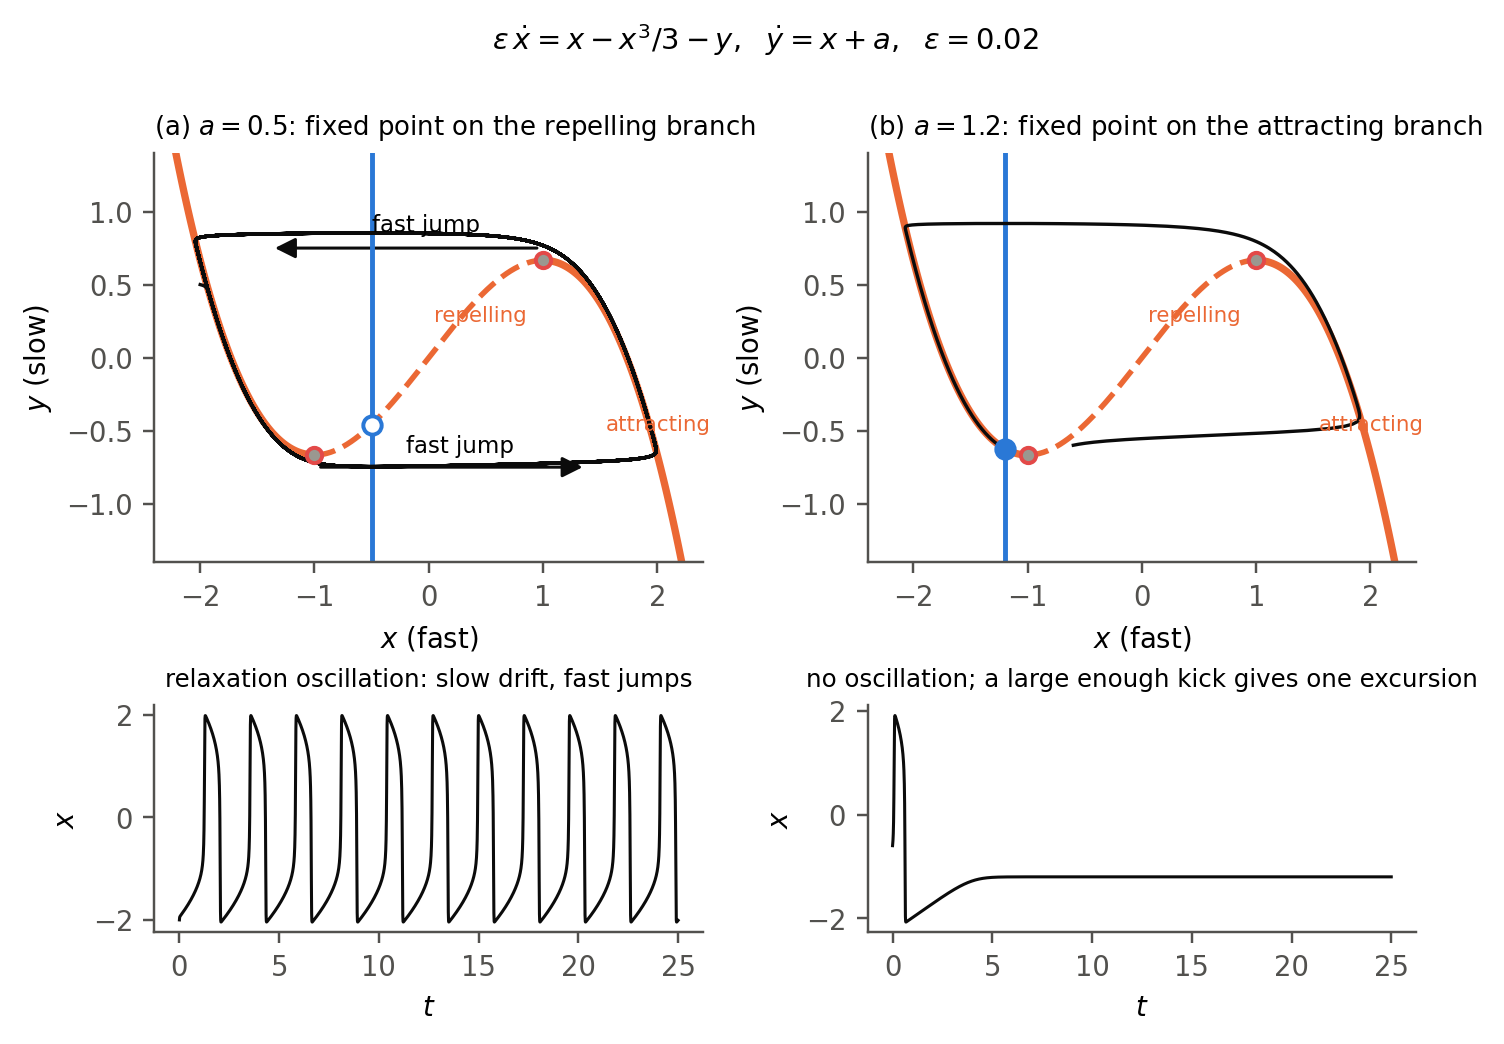
\includegraphics[width=\linewidth]{f10_slowfast.png}
\caption{Slow--fast system with a cubic critical manifold (orange; solid attracting, dashed repelling; grey dots: folds)
and a slow nullcline (blue). (a) Fixed point on the repelling branch: relaxation oscillation. (b) Fixed point on the
attracting branch, before the fold: excitable rest.}\label{fig:sf}
\end{figure}

\begin{recipe}[Reading a slow--fast phase plane]
\begin{enumerate}
\item Identify the fast variable (the one multiplied by $1/\eps$, or the one whose equation has the larger rate).
\item Draw the critical manifold (fast nullcline). Mark attracting ($\partial_x f<0$) and repelling ($\partial_x f>0$)
branches and the folds between them.
\item Draw the slow nullcline. Its intersection with $C_0$ is the fixed point.
\item Where is the fixed point? On an attracting branch: stable rest (excitable if close to a fold). On a repelling
branch: no stable rest, so relaxation oscillation. \textbf{Crossing a fold} is the transition.
\item Read the slow flow on each attracting branch from the sign of $g$ (which way $y$ moves), and follow it to a fold
or to the fixed point.
\item At a fold, jump horizontally (constant slow variable) to the next attracting branch.
\end{enumerate}
\end{recipe}

\section{Slow passage, period and duty cycle}
The period of a relaxation oscillation is dominated by the slow phases. On a branch $x(y)$ of $C_0$, the time spent is
$\int dy/g(x(y),y)$, which for the example gives $\int(1-x^2)\,dx/(x+a)$ along each branch. The fast jumps take a time of
order $\eps$. The fraction of the period spent on each branch (the duty cycle) is set by how fast $g$ moves the state on
that branch, i.e.\ by where the slow nullcline sits.

\begin{pitfall}[{The slow nullcline position is the control knob}]
In a slow--fast system, the qualitative behaviour (rest, excitable, oscillating) is decided by where the slow
nullcline crosses the critical manifold relative to its folds, not by the details of the fast dynamics. Moving the slow
nullcline across a fold is the whole story of the onset. This is exactly the role of $x_0$ in the Epileptor
(Chapter 11).
\end{pitfall}

%==========================================================================================
\chapter{Bursting: two time scales and two bifurcations}
%==========================================================================================
\section{Fast--slow dissection}
A \textbf{burster} alternates between active phases (fast oscillations) and quiet phases (rest). The standard model has
a fast subsystem with two or more variables (which can oscillate on its own) and one slow variable $z$:
\[
\dot{\mathbf x} = \mathbf f(\mathbf x, z),\qquad \dot z = \eps\, h(\mathbf x, z).
\]
\textbf{Dissection}: freeze $z$, compute the bifurcation diagram of the fast subsystem against $z$ (its fixed points and
limit cycles), and overlay the trajectory of the full system. The slow variable then moves the fast subsystem back and
forth along that diagram, through two bifurcations: one that starts the active phase and one that ends it. The pair
names the burster \cite{izhikevich}.

\section{Square-wave (fold/homoclinic) bursting}
The Hindmarsh--Rose model:
\[
\dot x = y - x^3 + 3x^2 - z + I,\qquad \dot y = 1 - 5x^2 - y,\qquad \dot z = r\,[s(x - x_R) - z],
\]
with $I=2$, $r=0.003$, $s=4$, $x_R=-1.6$ (Fig.~\ref{fig:burst}).

\begin{worked}[The fast subsystem of Hindmarsh--Rose]
With $z$ frozen, set $\dot y = 0$: $y = 1 - 5x^2$. Then $\dot x = 0$ gives the branch of fast fixed points
\[
z = -x^3 - 2x^2 + 1 + I .
\]
The fast Jacobian is $J = \begin{pmatrix} -3x^2 + 6x & 1\\ -10x & -1\end{pmatrix}$, so $\Delta = 3x^2 + 4x$ and
$\tau = -3x^2 + 6x - 1$.
\begin{itemize}
\item $\Delta < 0$ for $-4/3 < x < 0$: the middle branch is made of \textbf{saddles}.
\item For $x<-4/3$: $\Delta>0$, $\tau<0$: \textbf{stable rest} (lower branch).
\item $\Delta = 0$ at $x = -4/3$: a \textbf{fold} (saddle-node), at $z = I - 5/27 = 1.815$.
\item For $x>0$: $\Delta > 0$, and $\tau>0$ for $0.18<x<1.82$: \textbf{unstable focus} (upper branch), surrounded by a
stable limit cycle (green in Fig.~\ref{fig:burst}b).
\end{itemize}
\end{worked}

How the burst unfolds: during the quiet phase the state sits on the lower (rest) branch, where $s(x - x_R) < z$, so $z$
decreases. It slides left to the fold at $z = 1.815$, where the rest state disappears in a saddle-node: the state jumps
to the stable cycle and spikes. During spiking $x$ is high, so $z$ increases; the cycle moves right until it touches the
saddle branch, a \textbf{homoclinic bifurcation} of the fast subsystem: the cycle disappears and the state falls back to
rest. Fold onset, homoclinic offset: \emph{square-wave} or \emph{fold/homoclinic} bursting. The spike frequency slows
down at the end of each burst (logarithmic law), and the baseline shifts abruptly at onset.

\begin{figure}[H]\centering
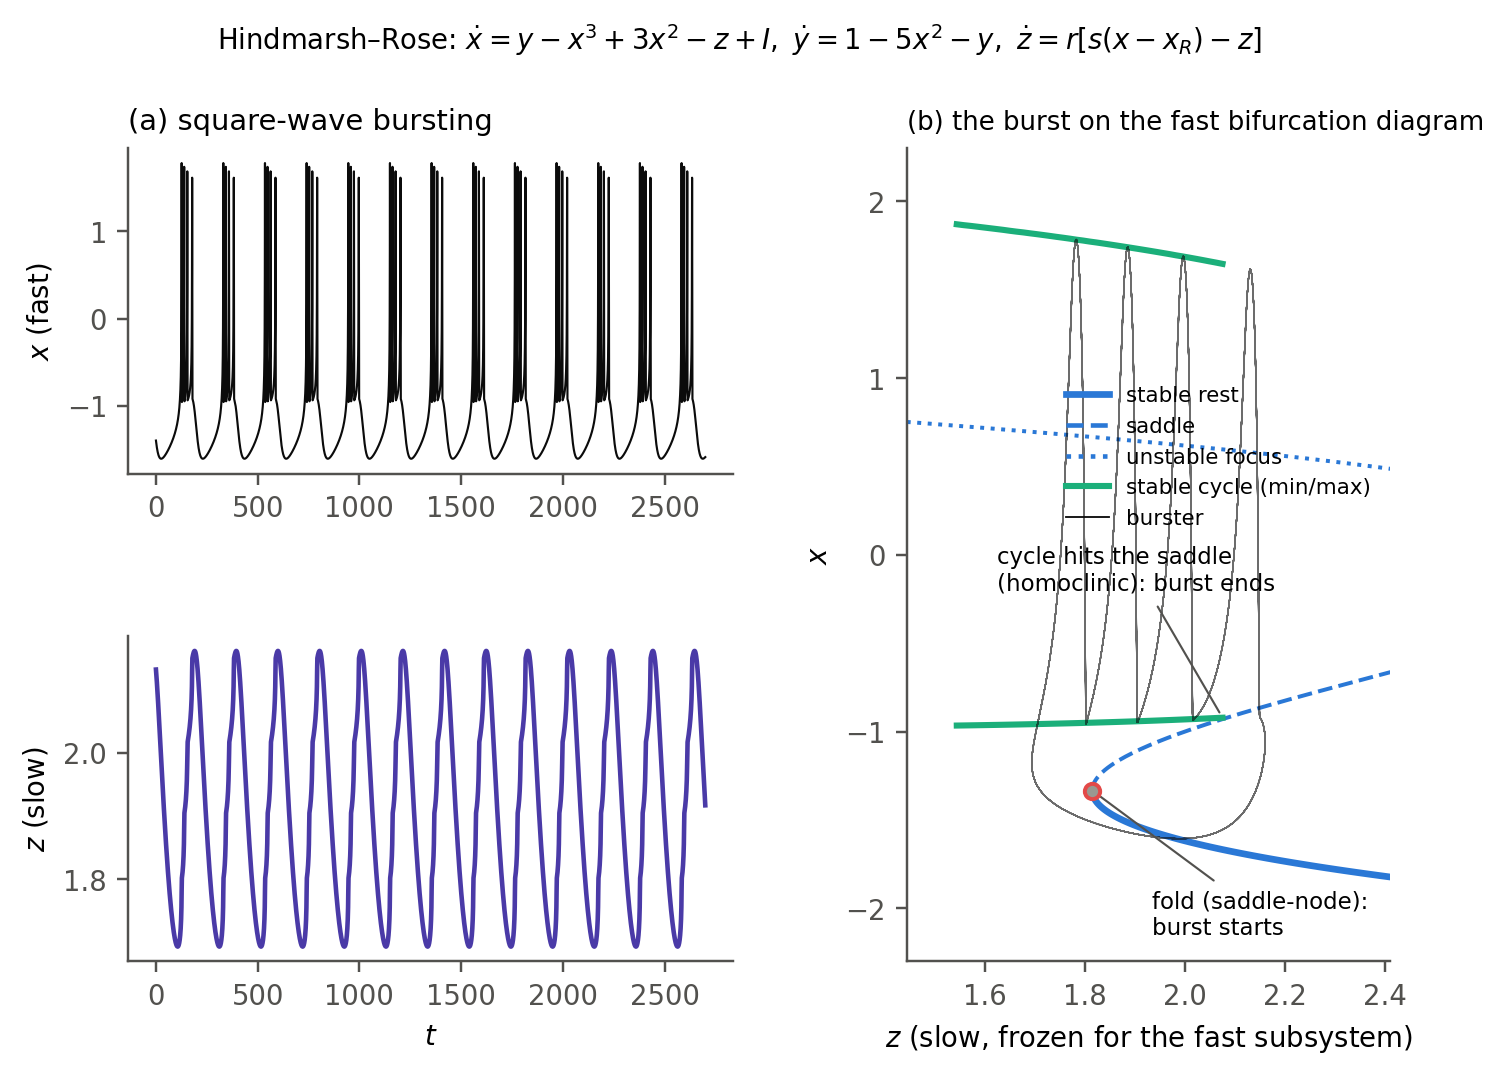
\includegraphics[width=\linewidth]{f11_bursting.png}
\caption{(a) Hindmarsh--Rose square-wave bursting: fast variable $x$ and slow variable $z$. (b) Dissection: fixed points
of the fast subsystem against $z$ (blue: solid stable, dashed saddle, dotted unstable focus), its stable cycle (green:
minimum and maximum of $x$) and the trajectory (black). The burst starts at the fold and ends where the cycle meets the
saddle branch.}\label{fig:burst}
\end{figure}

\begin{keyidea}[Why bursting is a hysteresis loop]
In the range of $z$ between the fold and the homoclinic point, the fast subsystem is \emph{bistable}: rest and spiking
coexist. The slow variable sweeps back and forth across this range, and because of the bistability, the fast subsystem
switches state only at the ends. The burster is a hysteresis loop of the fast subsystem driven by a slow negative
feedback ($z$ rises during spiking, falls at rest).
\end{keyidea}

Other burster classes come from other onset/offset pairs: SNIC/SNIC (parabolic or circle/circle bursting),
subcritical Hopf/fold of cycles (elliptic bursting, where spikes grow and shrink in amplitude), and so on.
Izhikevich's classification lists the combinations \cite{izhikevich2000}.

%==========================================================================================
\chapter{Checklist: identifying the behaviour from the equations}
%==========================================================================================
\begin{recipe}[From equations to behaviour]
\begin{enumerate}
\item \textbf{Time scales.} Is there a small parameter ($\eps$, $r$, $1/\tau$) multiplying one equation? Then treat the
system as slow--fast: fast subsystem first, slow nullcline second (Chapter 8).
\item \textbf{Fixed points.} Solve $f = g = 0$. Write the branch of fixed points as a function of the parameter; in
slow--fast systems, write the critical manifold.
\item \textbf{Jacobian.} Compute $\tau$ and $\Delta$ along the branch, as functions of the position on the branch.
\item \textbf{$\Delta$ changes sign?} Saddle-node (fold) if the branch turns back, i.e.\ $d\mu/dx = 0$ there. If the branch
continues straight through and exchanges stability with another, transcritical; if a symmetry produces two side
branches, pitchfork.
\item \textbf{$\tau$ changes sign with $\Delta>0$?} Hopf. Super or sub: compute $\ell_1$, or simulate just past it
(small growing amplitude vs immediate large amplitude, and bistability before).
\item \textbf{Cycles.} If a cycle exists (Poincaré--Bendixson), follow it with the parameter. Its period and amplitude
near the end tell how it dies: period $\sim1/\sqrt{\cdot}$ SNIC; period $\sim\ln$ homoclinic; amplitude $\to0$ Hopf;
both finite, fold of cycles.
\item \textbf{Bistability.} Two stable objects for the same parameter? Then expect hysteresis between two bifurcations.
\item \textbf{Slow variable.} If there is a slow variable, list the bifurcations of the fast subsystem it crosses, and
the direction it moves in each state. Two bifurcations bounding a bistable range plus a slow negative feedback give
bursting (or seizure-like) alternation.
\end{enumerate}
\end{recipe}

\begin{center}\small
\begin{tabular}{>{\raggedright}p{3.0cm}>{\raggedright}p{4.0cm}>{\raggedright}p{3.8cm}p{3.6cm}}
\toprule
bifurcation & condition from the equations & what it does & fingerprint \\
\midrule
saddle-node (fold) & $\Delta=0$ (one zero eigenvalue), branch turns back & node and saddle merge, vanish & critical slowing $\sqrt{\cdot}$; ghost time $\pi/\sqrt\mu$ \\
transcritical & $\Delta=0$, branch persists & exchange of stability & needs a fixed point that always exists \\
pitchfork & $\Delta=0$ + symmetry & one $\to$ three fixed points & needs $x\to-x$ symmetry \\
supercritical Hopf & $\tau=0$, $\Delta>0$, $\ell_1<0$ & stable cycle born at the focus & amplitude $\sqrt\mu$, finite frequency \\
subcritical Hopf & $\tau=0$, $\Delta>0$, $\ell_1>0$ & unstable cycle dies on the focus & jump, bistability, hysteresis \\
SNIC & saddle-node on a cycle & rest $\leftrightarrow$ cycle & frequency $\sqrt\mu$ \\
homoclinic & cycle touches a saddle (global) & cycle vanishes & period $\sim -\ln\mu$ \\
fold of cycles & two cycles merge (global) & cycle vanishes & nothing diverges \\
\bottomrule
\end{tabular}
\end{center}

\textbf{Codimension.} One-parameter families generically show only saddle-nodes and Hopf bifurcations among
local bifurcations of fixed points (``codimension one''). Points where two of these conditions meet need two
parameters (``codimension two'') and organise the two-parameter diagram: the \emph{cusp} (two folds meet; edge of the
hysteresis region), the \emph{Bautin} point ($\ell_1 = 0$, where a Hopf changes from super to sub), and the
\emph{Bogdanov--Takens} point (a saddle-node and a Hopf meet, with a homoclinic curve emanating from it).

%==========================================================================================
\chapter{Back to the Epileptor}
%==========================================================================================
This chapter only maps the vocabulary onto the model; the HSP--Epileptor report has the details.

\section{The 2D Epileptor is a slow--fast system}
\[
\dot x_1 = -x_1^3 - 2x_1^2 + 1 - z + I_{ext},\qquad \dot z = r\,[4(x_1 - x_0) - z],\qquad r = 0.00035 .
\]
$z$ is slow ($r\ll1$); $x_1$ is fast. This is Chapter 8 with $\eps = r$ and the variables renamed.
\begin{itemize}
\item \textbf{Critical manifold} (fast nullcline): $z = G(x_1) = -x_1^3 - 2x_1^2 + 1 + I_{ext}$, the same cubic as the
Hindmarsh--Rose fast subsystem (Chapter 9). Indeed, the Epileptor's first population \emph{is} a Hindmarsh--Rose-type
system, with $y_1$ eliminated.
\item \textbf{Branches.} $\partial_{x_1}\dot x_1 = G'(x_1) = -3x_1^2 - 4x_1 = -x_1(3x_1+4)$. It is negative for
$x_1<-4/3$ (lower, interictal branch: attracting) and for $x_1>0$ (upper, ictal branch: attracting), positive in between
(middle branch: repelling).
\item \textbf{Folds}: $G'=0$ at $x_1 = -4/3$ (bottom of the interictal branch, $z_{SN} = I_{ext} - 5/27 = 2.915$) and at
$x_1 = 0$ (top of the ictal branch, $z = 1 + I_{ext} = 4.1$). The ``fold'' of the report is the first one: the onset.
\item \textbf{Slow nullcline}: $z = 4(x_1 - x_0)$, a line of slope 4. $x_0$ shifts it sideways: it is the control knob
of Chapter 8.
\end{itemize}

\begin{figure}[H]\centering
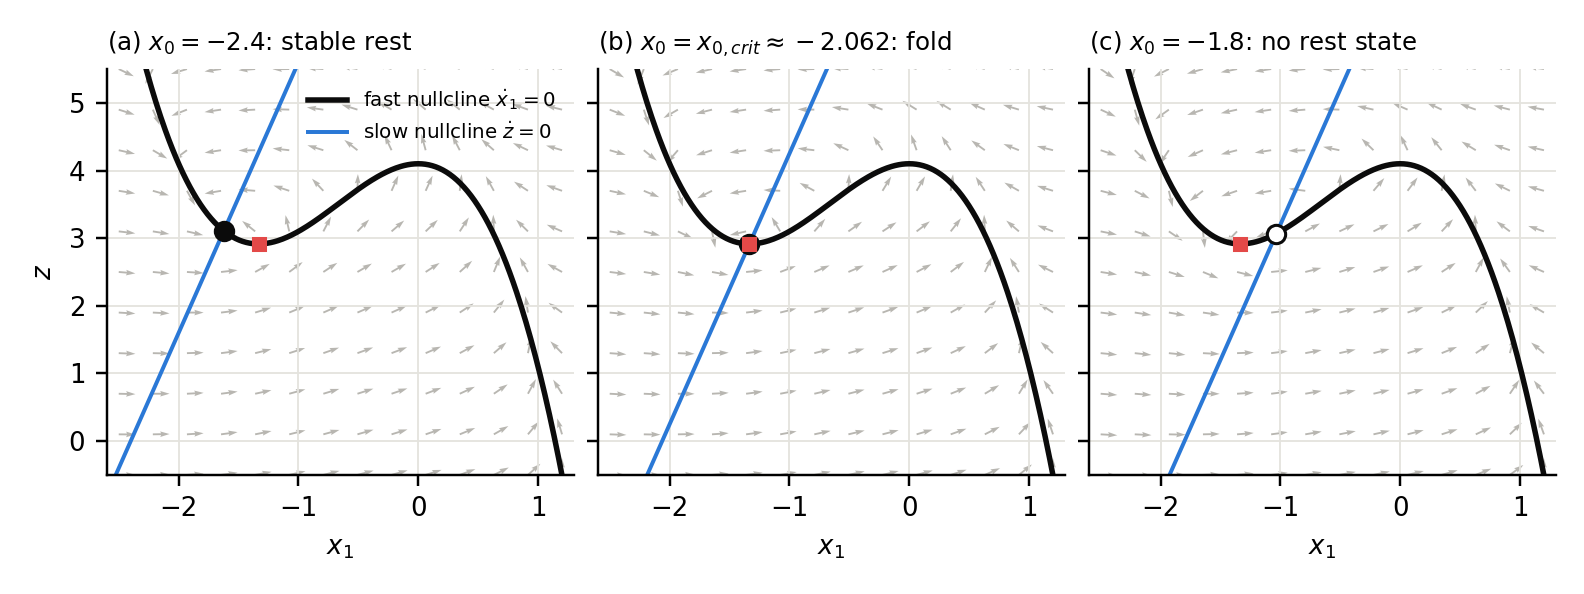
\includegraphics[width=\linewidth]{th_phase_planes.png}
\caption{2D Epileptor phase planes (from the report). (a) The slow nullcline crosses the interictal branch before the
fold: stable rest. (b) It passes through the fold: the critical value $x_{0,crit}$. (c) It crosses the repelling middle
branch: no stable rest, relaxation oscillation (seizures).}
\end{figure}

\section{Reading it with the checklist}
\begin{enumerate}
\item \textbf{Time scales}: slow--fast, $\eps = r$.
\item \textbf{Fixed point}: one intersection of the line with the cubic, for every $x_0$ (slope 4 is steeper than the
cubic anywhere, so they cross once).
\item \textbf{Jacobian}: $J = \begin{pmatrix} G'(x_1^*) & -1\\ 4r & -r\end{pmatrix}$, $\Delta = r\,(3x_1^{*2} + 4x_1^* + 4) >
0$ always (the quadratic has no real root), $\tau = G'(x_1^*) - r$.
\item \textbf{$\Delta$} never changes sign: no saddle-node of the full system.
\item \textbf{$\tau$} changes sign when $G'(x_1^*) = r$, i.e.\ just past the fold: a Hopf bifurcation, singular because $r$
is tiny, so in practice an abrupt onset of large relaxation oscillations at $x_0\approx x_{0,crit}$ (Chapter 8,
canard explosion).
\item \textbf{Fast subsystem} ($z$ frozen, 1D): two folds (saddle-nodes) at $z_{SN}$ and $z = 4.1$, bistability between
them, and a slow negative feedback $z$: a hysteresis loop of the fast subsystem, i.e.\ a seizure is one turn of the loop
(Fig.~\ref{fig:epirelax}).
\end{enumerate}

\begin{figure}[H]\centering
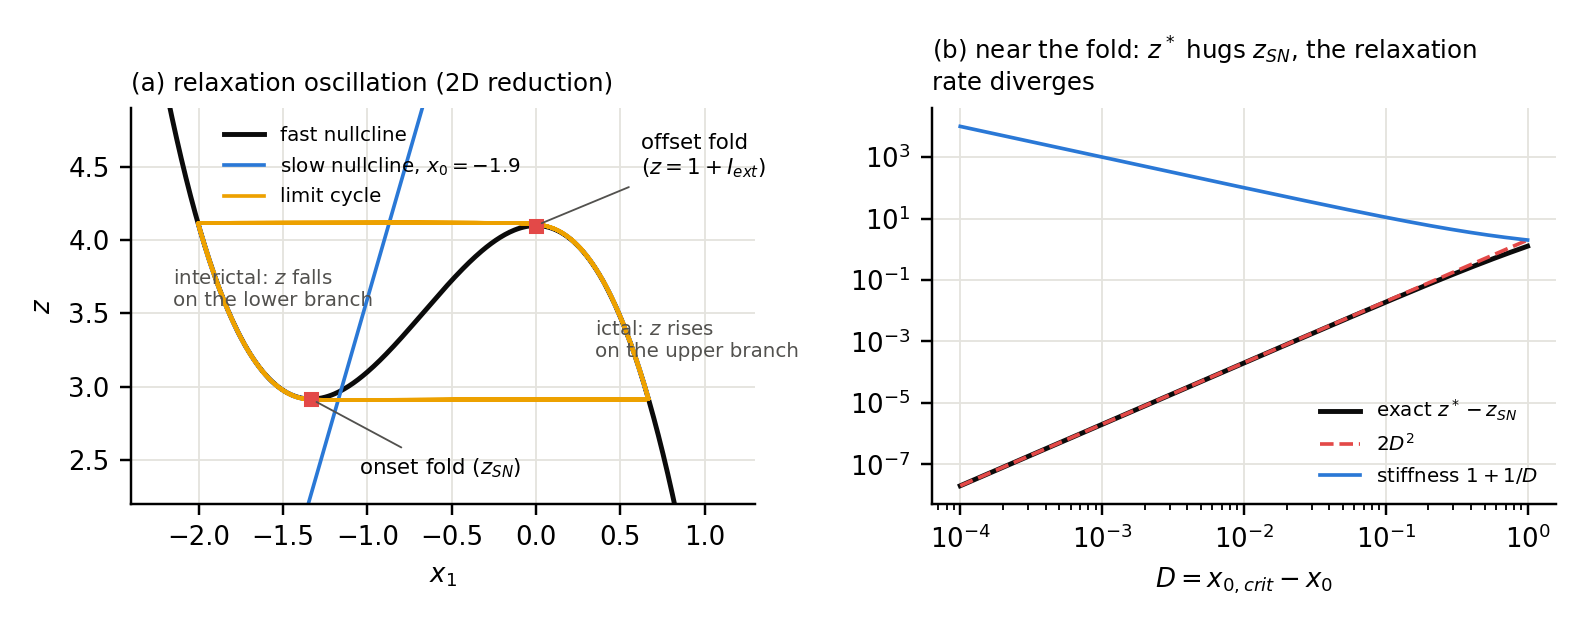
\includegraphics[width=\linewidth]{th_relaxation.png}
\caption{(a) The 2D Epileptor relaxation cycle: slow fall of $z$ on the interictal branch, jump at the onset fold, slow
rise on the ictal branch, jump back at the offset fold. (b) Near the fold, the fixed point sits only $2D^2$ above $z_{SN}$
and its relaxation rate grows as $1/D$: critical slowing down of the saddle-node.}\label{fig:epirelax}
\end{figure}

\section{The same thing as a ball on a tilting board}
In the landscape picture of Fig.~\ref{fig:land} (bottom), the fast nullcline is simply the map of where the valleys and the
crest of the landscape $V(x_1)$ are, for every $z$:
\begin{center}\small
\begin{tabular}{lll}
\toprule
fast nullcline & landscape at fixed $z$ & the ball \\
\midrule
left (interictal) branch, attracting & floor of the left valley & at rest \\
middle branch, repelling & crest between the valleys & on the threshold \\
right (ictal) branch, attracting & floor of the right valley & seizing \\
folds ($G'=0$) & a valley merging with the crest & the valley vanishes, the ball rolls \\
\bottomrule
\end{tabular}
\end{center}
The slow variable $z$ is a hand that tilts the board very slowly and reacts to where the ball is: while the ball is in the
left valley it tilts one way ($z$ decreases, if $x_0$ is past the threshold), while it is in the right valley the other way
($z$ increases). ``The state follows the fast nullcline'' means the ball stays at the bottom of its valley while the valley
moves. Between the two folds both valleys exist (bistability), and which one the ball is in depends on its history
(hysteresis). The excitability $x_0$ sets how far the hand tilts while the ball rests: for $x_0<x_{0,crit}$ it stops before
the left valley disappears, so the ball stays; for $x_0>x_{0,crit}$ it keeps tilting until the valley is gone, so the
seizures repeat. HSP slowly turns that knob.

\section{Onset and offset in the full Epileptor}
In the full model, the fast subsystem (population 1) has two variables and can oscillate. Its onset is the saddle-node
(fold) of the rest state, as in the 2D reduction, but its offset is a \textbf{homoclinic} bifurcation: the seizure
oscillation ends when it touches the saddle branch, exactly as in Hindmarsh--Rose. Onset by fold, offset by homoclinic:
the Epileptor is a \textbf{square-wave burster} (Chapter 9). Its clinical fingerprints follow from the table of Chapter 6:
an abrupt baseline (DC) shift at onset (saddle-node), and a logarithmic slowing of the discharges before the end
(homoclinic) \cite{jirsa2014}.

\section{Where HSP enters}
In the HSP mapping, $x_0$ is no longer a constant but a slow variable set by the excitatory gain,
$x_0 = x_{0,crit} + \ln(k_E/k_E^c)$. This adds a third, even slower time scale. Between high-risk periods, HSP moves the
slow nullcline towards the onset fold (approaching the saddle-node, with the critical slowing down of
Fig.~\ref{fig:epirelax}b); a high-risk period starts when it reaches the fold; afterwards HSP throws it far back. In the
language of this text: HSP is a slow parameter drift that carries the Epileptor back and forth across its saddle-node,
and $z$ is the faster negative feedback that would produce the individual seizures while $x_0$ is past it.

%==========================================================================================
\appendix
\chapter{Exercises}
%==========================================================================================
\begin{enumerate}[label=\textbf{\arabic*.}]
\item Find and classify the fixed points of $\dot x = r - x - e^{-x}$ as $r$ varies. At what $r$ is there a saddle-node?
\item For $\dot x = \mu x - x^2$, sketch the bifurcation diagram and explain why the fixed point $x=0$ exists for all
$\mu$.
\item Classify the fixed point of $\dot x = -x + 2y$, $\dot y = -3x - y$.
\item For $\dot x = y$, $\dot y = -x + \mu y - y^3$ (van der Pol type), find the Hopf bifurcation and decide whether it
is supercritical.
\item In FitzHugh--Nagumo with $b=0.8$, $\eps=0.08$, explain from $\Delta$ why there is never a saddle-node.
\item A neuron starts firing at very low frequency, and the frequency grows as the current increases. What is the onset
bifurcation? What if it starts at a finite frequency with a small amplitude?
\item In $\eps\dot x = x - x^3/3 - y$, $\dot y = x + a$, for which values of $a$ does the system oscillate? Draw the
relaxation cycle for $a=0$.
\item In the 2D Epileptor, show that $x_{0,crit} = -4/3 - z_{SN}/4$, and compute it for $I_{ext}=3.1$.
\item Why can a one-dimensional fast subsystem (the 2D Epileptor at fixed $z$) not have a homoclinic offset?
\end{enumerate}

\section*{Solutions}
\begin{enumerate}[label=\textbf{\arabic*.}]
\item Fixed points: $r = x + e^{-x}$. The right side has a minimum at $x=0$, value 1. So: no fixed point for $r<1$, a
saddle-node at $r=1$, $x=0$, and two fixed points for $r>1$. $f'(x) = -1 + e^{-x}$: negative for $x>0$ (stable), positive
for $x<0$ (unstable).
\item Fixed points 0 and $\mu$; $f' = \mu - 2x$, so 0 is stable for $\mu<0$ and $\mu$ is stable for $\mu>0$. $x=0$ always
solves $\mu x - x^2 = 0$ because the right side has a factor $x$ (a population that is zero stays zero): transcritical.
\item $\tau = -2$, $\Delta = 1 + 6 = 7$, $\tau^2 - 4\Delta = -24 < 0$: stable focus.
\item At the origin $J = \begin{pmatrix}0&1\\-1&\mu\end{pmatrix}$, $\tau = \mu$, $\Delta = 1$: Hopf at $\mu = 0$ with
$\omega=1$. At $\mu=0$ the linear part is $\dot u = v$, $\dot v = -u$; with $u\to v$, $v\to u$ it becomes the rotation
form with $G = 0$, $F = -u^3$ in the swapped variables, so $\ell_1 = F_{uuu}/16 = -6/16<0$: supercritical. Simulation:
amplitude grows like $\sqrt\mu$.
\item $\Delta = \eps[1 - b(1 - x^{*2})]$ vanishes only if $1 - x^{*2} = 1/b = 1.25$, i.e.\ $x^{*2} = -0.25$: impossible. The
$y$-nullcline (slope $1/b = 1.25$) is steeper than the cubic's maximum slope (1), so they always cross once.
\item Low frequency at onset: SNIC (frequency $\propto\sqrt{I - I_c}$). Finite frequency, small amplitude: supercritical
Hopf.
\item The fixed point $x^* = -a$ is on the repelling branch for $|a|<1$: oscillation for $-1<a<1$. For $a=0$: slide down
the left branch from $(-2, 2/3)$ to the fold $(-1,-2/3)$, jump to $(2,-2/3)$, slide up to the fold $(1, 2/3)$, jump back to
$(-2, 2/3)$.
\item At the critical value the slow nullcline $z = 4(x_1 - x_0)$ passes through the fold $(-4/3, z_{SN})$:
$z_{SN} = 4(-4/3 - x_0)$, so $x_0 = -4/3 - z_{SN}/4$. With $z_{SN} = 3.1 - 5/27 = 2.9148$, $x_{0,crit} = -2.062$.
\item A homoclinic orbit needs a closed loop through a saddle, and a cycle needs at least two dimensions. A
one-dimensional flow has neither cycles nor saddles (only stable and unstable points on a line), so the 2D Epileptor can
only end a seizure through the second fold, where the ictal branch ends.
\end{enumerate}

\begin{thebibliography}{9}\small
\bibitem{strogatz} S.~H. Strogatz. \emph{Nonlinear Dynamics and Chaos}, 2nd ed. Westview Press, 2015.
\bibitem{izhikevich} E.~M. Izhikevich. \emph{Dynamical Systems in Neuroscience: The Geometry of Excitability and
Bursting}. MIT Press, 2007.
\bibitem{izhikevich2000} E.~M. Izhikevich. Neural excitability, spiking and bursting. \emph{Int.\ J.\ Bifurcation and
Chaos} 10:1171--1266, 2000.
\bibitem{kuznetsov} Yu.~A. Kuznetsov. \emph{Elements of Applied Bifurcation Theory}, 3rd ed. Springer, 2004.
\bibitem{guckenheimer} J.~Guckenheimer, P.~Holmes. \emph{Nonlinear Oscillations, Dynamical Systems, and Bifurcations
of Vector Fields}. Springer, 1983.
\bibitem{kuehn} C.~Kuehn. \emph{Multiple Time Scale Dynamics}. Springer, 2015.
\bibitem{jirsa2014} V.~K. Jirsa, W.~C. Stacey, P.~P. Quilichini, A.~I. Ivanov, C.~Bernard. On the nature of seizure
dynamics. \emph{Brain} 137:2210--2230, 2014.
\end{thebibliography}
\end{document}
